\documentclass[]{final_report}
\usepackage{graphicx}
\usepackage{hyperref}
\usepackage{sectsty}
\usepackage{subcaption}
\usepackage{listings}
\usepackage{csquotes}


%%%%%%%%%%%%%%%%%%%%%%
%%% Input project details
\def\studentname{Vinay Kakkar}
\def\reportyear{2023}
\def\projecttitle{Structural Bioinformatics Framework using a MapReduce formalism}
\def\supervisorname{Hugh P. Shanahan}
\def\degree{MSc in Computer Science with a Year In Industry}
\def\fullOrHalfUnit{Full Unit} % indicate if you are doing the project as a Full Unit or Half Unit
\def\finalOrInterim{Final Report} % indicate if this document is your Final Report or Interim Report
\sectionfont{\clearpage}
\begin{document}

\maketitle

\newtheorem{definition}{Definition}[section]
\renewcommand\thesection{\arabic{section}}

\begin{abstract}
    Structural bioinformatics is a rapidly growing field that aims to understand biological processes at the molecular level. This dissertation proposes, a novel framework for structural bioinformatics using a MapReduce formalism. Our framework allows for efficient processing of large-scale structural data by distributing computation across a cluster of computers. We demonstrate the effectiveness of our approach through benchmarking and comparisons with current implemented solutions. When using more worker nodes with more cores it shows a vast improvement when compared to singular execution. Our framework not only provides faster computation but also offers enhanced scalability and fault tolerance, making it a valuable tool for large-scale structural bioinformatics analyses. Furthermore, we highlight the potential of our framework for facilitating collaboration and data sharing among researchers, which is crucial for advancing our understanding of complex biological systems. Overall, our proposed framework presents a significant step forward in the field of structural bioinformatics, enabling the efficient and scalable analysis of complex structural data. By reducing processing time and enhancing data retrieval. 
\end{abstract}

\renewcommand{\abstractname}{Acknowledgements}
\begin{abstract}
    I would like to express my sincere gratitude to my supervisor Hugh Shanahan, for his support, guidance, and patience throughout my dissertation journey. I would like to express my appreciation to my family and friends for their constant support and understanding throughout my dissertation. Finally, to all others who have been a part of this journey, I am deeply grateful for your support.
\end{abstract}

\section{Motivation}
The need for structural bioinformatics is growing vastly more specifically, for its role in understanding biological processes and in the development of new drugs. As a result analysing and interpreting complex data such as the three-dimensional structures of proteins, DNA, and other macromolecules has taken a toll. Due to the size and complexity of these datasets increasing it has been demanding more efficient and scalable computational tools to perform analysis and processing tools.

MapReduce provides a promising approach to addressing this challenge. It is a programming model for large-scale data processing in distributed computing environments, which enables parallel processing of large datasets across multiple nodes in a cluster. This can significantly improve the speed and efficiency of data analysis tasks.

In this project, we present a structural bioinformatics framework that performs a MapReduce formalism on structural data to perform analysis on protein structure data. This framework is based on a distributed computing architecture that allows for the parallel processing of protein structures protein-protein interactions or molecular structures.

With a series of experiments on protein structure data sets, we can demonstrate the effectiveness of our framework. As a result, showing that our approach can significantly reduce the time and resources required for complex bioinformatics tasks. Moreover, the results demonstrate the potential of MapReduce-based approaches have on accelerating the analysis of large-scale structural data and aiding in drug development and biological research.

By enabling researchers to carry out intricate studies on big datasets in a parallel, distributed manner, this approach has the potential to fundamentally alter the field. This will ultimately save precious time and computational resources, allowing researchers to advance their studies of protein structures more quickly and maybe leading to new discoveries in the field.
\clearpage

\section{Aims and Objectives}
\subsection{Aim provided in the Project Description}
"The aim of this project is to be provide a framework where large numbers of protein structures can be analysed using a user-provided executable in the MapReduce formalism."

\subsubsection{Aim}
Analysing protein structures can provide insights into their properties and interactions with other molecules. However, analysing large numbers of protein structures can be computationally intensive, requiring significant computational resources and time. Thus, the aim is to provide a framework that allows for the analysis of large numbers of protein structures using a MapReduce formalism.

\textbf{\textit{MapReduce:}} is a programming model for processing and generating large data sets. Allowing for parallel processing of data across multiple nodes in a cluster, making it well-suited for analysing large datasets.

More specifically the aim is to develop a framework that can take a user-provided executable and apply it to a large number of protein structures in a parallel, distributed manner using MapReduce. This will enable researchers to perform complex analyses on large datasets of protein structures more efficiently, saving time and computational resources. Essentially enabling researchers to analyse large numbers of protein structures more quickly and effectively than before.
\clearpage

\subsection{Objectives}

To achieve the aim of the project, the following objectives have been formulated:

\begin{enumerate}
    \item Develop a software framework that supports the MapReduce formalism and can process large numbers of protein structures.
    \item Implement a distributed computing system using MapReduce to parallelize protein structure analysis across multiple computing nodes.
    \item Optimize the software framework to reduce the processing time required for protein structure analysis.
    \item Design an interface that allows users to manipulate the PDBs that are being passed into the executable for protein structure analysis.
    \item Ensure the software framework is scalable and can handle increasingly large datasets.
    \item Ensure the software framework can be easily updated to keep pace with advancements in protein structure analysis techniques and computing technology.
    \item Provide documentation and user support to enable researchers to use the software framework effectively
\end{enumerate}
\clearpage

\subsection{Rationale for Objectives}

\subsubsection{MapReduce Framework for Protein Analysis}

\begin{displayquote}
    Develop a software framework that supports the MapReduce formalism and can process large numbers of protein structures.
\end{displayquote}

Frameworks that can process vast volumes of data quickly are required due to the growth in the amount of data created in structural bioinformatics. A distributed computer cluster can process big datasets with the help of the MapReduce programming methodology. By breaking up the data into smaller chunks, which are subsequently analysed simultaneously across several computing nodes, it enables parallel processing of the data. Because MapReduce can handle the dispersed processing of data across a cluster of computers, designing software that supports it enables the efficient processing of numerous protein structures.

\subsubsection{Parallelized Protein Analysis with MapReduce}

\begin{displayquote}
    Implement a distributed computing system using MapReduce to parallelize protein structure analysis across multiple computing nodes.
\end{displayquote}

Analysis of protein structures requires a lot of computing and can take a long time to accomplish on a single machine. The study can be parallelized across numerous processing nodes by using MapReduce to construct a distributed computing system, greatly lowering the amount of time needed to process the data. This makes it possible to analyse protein structures more quickly, which is crucial in research areas like drug discovery.

\subsubsection{Optimization for Faster Protein Analysis}

\begin{displayquote}
    Optimize the software framework to reduce the processing time required for protein structure analysis.
\end{displayquote}

Even with a distributed computing system, the processing time required for protein structure analysis can be significant. Thus, the software framework must be optimized to reduce the processing time required for protein structure analysis. This can be achieved by improving the efficiency of the algorithms used in the analysis, minimizing the amount of data transferred between nodes, and optimizing the hardware used in the computing cluster. Optimizing the software framework ensures that protein structure analysis can be done as quickly and efficiently as possible.
\clearpage

\subsubsection{User Interface for Protein Analysis}

\begin{displayquote}
    Design an interface that allows users to manipulate the pdbs that are being passed into the executable for protein structure analysis.
\end{displayquote}

As the framework revolves around using and manipulating PDB file. An interface for manipulating the input data is necessary to provide users with the flexibility to customize their protein structure analysis. This interface should be intuitive and easy to use, allowing researchers to select the protein structures they want to analyze and adjust the analysis parameters as needed. Providing this interface ensures that researchers can tailor the analysis to their specific needs and allows for greater flexibility in the types of analysis that can be performed.

\subsubsection{Scalable Data Handling for Protein Analysis}

\begin{displayquote}
    Ensure the software framework is scalable and can handle increasingly large datasets.
\end{displayquote}

As the size of protein structure datasets continues to increase, it is essential that the software framework can scale to handle this growth without a significant decrease in performance. The system should be designed to handle datasets of various sizes and be able to scale up or down based on the demands of the analysis. This ensures that the software framework can handle the ever-increasing amounts of data generated by modern research techniques.
\clearpage

\subsubsection{Upgradable Framework for Advanced Analysis}

\begin{displayquote}
    Ensure the software framework can be eaisly updated to keep pace with advancements in protein structure analysis techniques and computing technology.
\end{displayquote}

The software framework must be able to keep up with the most recent developments as protein structure analysis continues to develop. This means that in order to make it simple to incorporate new analysis approaches, the framework should be created to be modular and extendable. High-performance computing clusters, the most recent computing technologies, should be incorporated into its design. This makes sure that if new research methodologies are created, the software framework may continue to be applicable and useful.

\subsubsection{User Support for Protein Analysis Software}

\begin{displayquote}
    Provide documentation and user support to enable researchers to use the software framework effectively.
\end{displayquote}

To ensure that researchers can use the software framework effectively, comprehensive documentation and user support are essential. This includes detailed documentation on how to install and configure the software, as well as guides on how to use the various functions provided by the framework. Providing documentation and user support helps to ensure that researchers can use the framework for their research purposes and obtain accurate results from their protein structure analyses.

\subsubsection{Further Objective: Integrate API for PDB access}

\begin{displayquote}
    Integrate a PDB file download and search from the RCSB API for efficient data access.
\end{displayquote}

The PDB bank is a crucial tool for structural bioinformatics since it enables researchers to access and search for specific PDB files that are pertinent to their work. Researchers can download and search for PDB files by integrating an API, which makes it simpler to obtain and analyse the pertinent structural data. Researchers will be able to use the framework as a result, improving research process effectiveness. Also, making this data more readily available to academics can encourage data sharing and collaboration, which will advance research in the field of structural bioinformatics.

\clearpage

\subsection{Conclusion: Aims and Objectives}

In conclusion, this project aims to develop a software framework using MapReduce formalism that can analyse large numbers of protein structures efficiently utilising a user-provided executable. To achieve this aim, several objectives have been formulated, including developing a software framework that supports the MapReduce formalism, implementing a distributed computing system for parallelizing protein structure analysis, optimizing the software framework, designing an interface for manipulating the input data, ensuring scalability of the software framework and integrating an API for PDB access. These objectives will ensure that researchers can perform complex analyses on large datasets of protein structures more efficiently, saving time and computational resources. By achieving these objectives, this project will make a significant contribution to the field of structural bioinformatics, enabling researchers to analyze large numbers of protein structures more quickly and effectively than before.

\section{Protien Structures, PDB Bank and Big Data Frameworks}
\subsection{Protein Structures}
\subsubsection{Introduction}

Amino acids are molecules that when combined forms proteins. All of the 20 amino acids, see table~\ref{Amino acids} have in common a central carbon atom which is attached to a hydrogen atom, an amino group, and a carboxyl group~\cite{branden_introduction_1998}.

Proteins are responsible for catalysing most of the chemical reactions in cells. They can function as enzymes catalysing a wide variety of reactions important for life and thus also important for the structure of living systems such as proteins involved in the cytoskeleton. The size of protein can vary ~\cite{zvelebil_understanding_2008}.

\begin{definition}[Catalysing]
    Catalysing is to make a chemical reaction happen or happen more quickly by acting as a catalyst.
\end{definition}

\begin{definition}[Cytoskeleton]
    A dynamic network of interlinking protein filaments present in the cytoplasm of all cells~\cite{zvelebil_understanding_2008}. 
\end{definition}

\subsubsection{Primary, Secondary, Tertiary and Quaternary Structure}

Please refer to~\ref{fig:levels of protein structure.} for a visual representation.

The \textbf{primary structure} of a peptide or protein is the linear sequence of its amino acids. It is read and written from the amino-terminal to the carboxyl-terminal end.~\cite{sun_overview_2004}.

The \textbf{secondary structure} refers to the local arrangement of a peptide chain. Where several common secondary structures have been identified in proteins~\cite{sun_overview_2004}.

\textbf{Tertiary structure} is a three-dimensional structure of a protein the formation is built up of bonds and interactions that serve to change the shape of the overall protein~\cite{godbey_chapter_2022}.

The \textbf{quaternary structure} of a protein is built-up of several protein chains/subunits. Each of the subunits has its primary, secondary, and tertiary structure~\cite{ouellette_14_2015}.
\clearpage

\subsubsection{Considering Protein structure on several different levels}

The fold of the protein plays part in determining the way the protein will function, and also whether it will function correctly. As there are Protein structures on different levels we need to consider the analysis of protein structure by experimental techniques such as X-ray crystallography, nuclear magnetic resonance, and RNAseq which show that proteins adopt distinct structural elements~\cite{zvelebil_understanding_2008}.
\vspace{80px}


 
\begin{figure}[h]
    \centering
    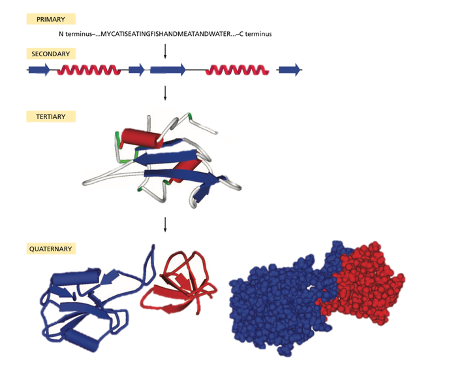
\includegraphics[width=0.5\textwidth]{Protein Structure.png}
    \caption{\label{fig:levels of protein structure.}From the sequence alone, the primary structure to secondary structure, to tertiary structure(3D), to finally quaternary structure found when several tertiary structures form a multisubunit complex~\cite{zvelebil_understanding_2008}.}
\end{figure}
\clearpage

\subsubsection{Amino Acids}

Sequence of amino acids~\ref{Amino acids} will build up the linear protein chain~\cite{zvelebil_understanding_2008}. Amino acids are different from each other due to their side chains and due to this the functional properties of various different proteins are different~\cite{zvelebil_understanding_2008}. You can see the amino acids grouped here~\ref{Amino acids}.
\vspace{80px}

\begin{table}[h!]
    \begin{center}\label{tab:Amino acids}
        \begin{tabular}{l|c|r}
        Amino acid & Three-letter code & One-letter code\\
        \hline
        \\
        Glycine & Gly & G\\
        Alanine & Ala & A\\
        Valine & Val & V\\
        Leucine & Leu & L\\
        Isoleucine & Ile & I\\
        Proline & Pro & P\\
        Phenylalanine & Phe & F\\
        Methionine & Met & M\\
        Tryptophan & Trp & W\\
        Cysteine & Cys & C\\
        \\
        \hline
        \\
        Asparagine & Asn & N\\
        Glutamine & Gln & Q\\
        Serine & Ser & S\\
        Threonine & Thr & T\\
        Tyrosine & Tyr & Y\\
        \\
        \hline
        \\
        Aspartic acid & Asp & D\\
        Glutamic acid & Glu & E\\
        \\
        \hline
        \\
        Histidine & His & H\\
        Lysine & Lys & K\\
        Arginine & Arg & R\\
        \end{tabular}
        \caption{\label{Amino acids}The 20 amino acids. The amino acid name, the three-letter code, and the one-letter code are given. The Amino acids are split up into Nonpolar, Polar, Acidic and Basic respectfully}
    \end{center}
\end{table}
\clearpage

\subsection{Large Scale Experssion}

Gene expression begins when genes are transcribed into messenger RNAs, which are then translated to produce proteins. 

Total gene expression in cultured cells or a tissue sample can be detected in three main ways:

\begin{enumerate}
    \item DNA microarray technology.
    \item Two-dimensional Gel electrophoresis or Chromatography.
    \item RNAseq
\end{enumerate}

Both DNA microarray technology and Two-dimensional Gel electrophoresis, produce enormous amounts of raw data~\cite{zvelebil_understanding_2008} due to this, many proteins currently evade high-resolution structure determination.


\subsubsection{Structural mass spectrometry}
Structural mass spectrometry is a powerful approach used to determine the 3D structure of biological protiens it has nearly an unlimited size constraint and speed. Although the data provided by mass spectrometry is vague for full high-resolution structure elucidation, structural mass spectrometry can be used to examine the size, solvent accessibility, and topography of proteins~\cite{limpikirati_covalent_2018}~\cite{liu_mass_2020}.

We can have computational methods that aid experimental technique intending to elucidate protein structures~\cite{seffernick_hybrid_2020}~\cite{leman_macromolecular_2020}. Software packages can be used to combine data with advanced structure sampling and scoring techniques. Computational tools for protein structure modeling, include the Rosetta software suite~\cite{leman_macromolecular_2020}~\cite{alford_rosetta_2017}, I-TASSER~\cite{yang_i-tasser_2015}, Phyre2~\cite{kelley_phyre2_2015}, Integrative Modeling Platform~\cite{russel_putting_2012}, HADDOCK~\cite{dominguez_haddock_2003}, and MODELLER~\cite{eswar_comparative_2006}~\cite{biehn_protein_2022}.

\clearpage
\subsubsection{Large Scale Gene Expression}

Genome DNA microarray experiments produce large amounts of data that can be computationally heavy on where methods can yield alternative conclusions from increasing the computational effort.

The goal of these experiments is to determine biological or functional meaning from the lists of genes, either by:

\begin{enumerate}
    \item Identify critical genes that are responsible for a biological effect.
    \item Find patterns within the genes that point to an underlying biological process.
\end{enumerate}
\cite{zvelebil_understanding_2008}

\begin{figure}[ht]
    \centering
    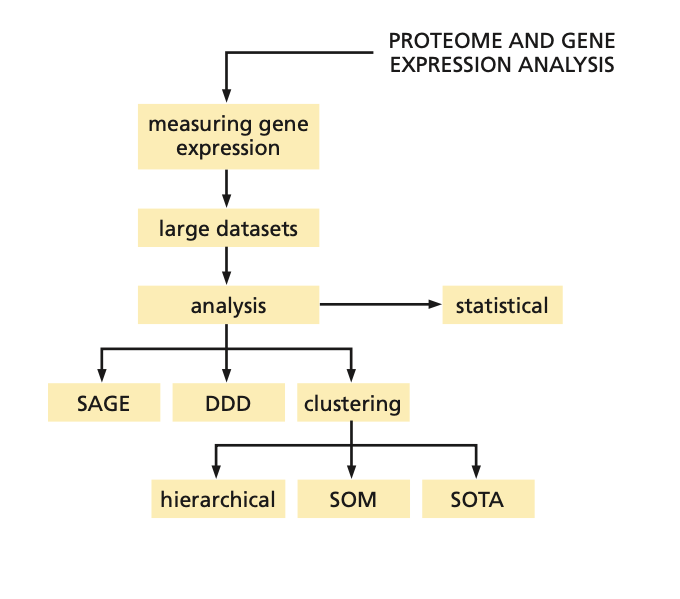
\includegraphics[width=0.5\textwidth]{Gene Expresion.png}
    \caption{\label{fig:Gene Expression}Describing Common experimental aspects of gene expression and of the analysis of the resulting data~\cite{zvelebil_understanding_2008}.}
\end{figure}

\clearpage

\subsubsection{Serial analysis of gene expression}

Serial analysis of gene expression is the alternative compared to microarrays when trying to investigate patterns of gene expression.

\begin{figure}[!h]
    \centering
    \begin{subfigure}[t]{.45\textwidth}
        \centering
        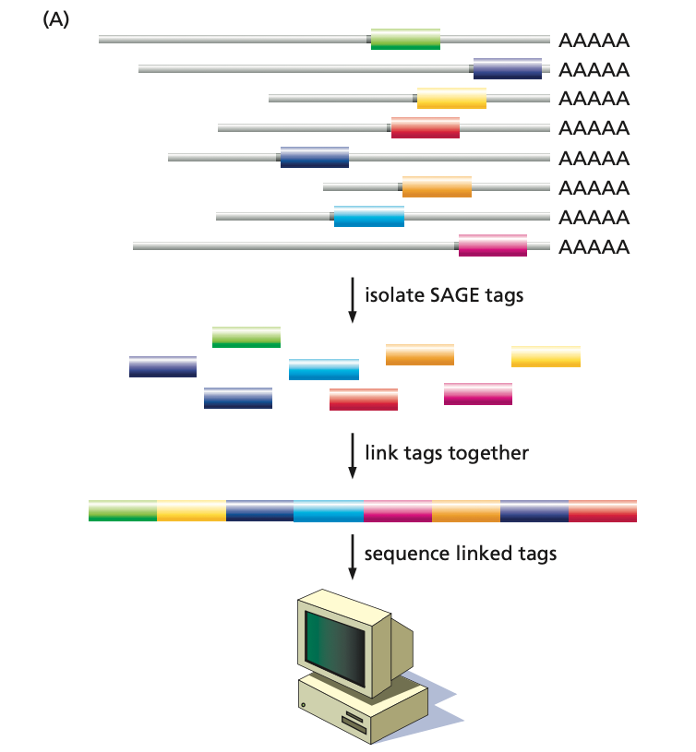
\includegraphics[width=0.9\textwidth]{SAGE1.png}
        \caption{}
        \label{fig:SAGE1} 
    \end{subfigure}
    \begin{subfigure}[t]{.45\textwidth}
       \centering
       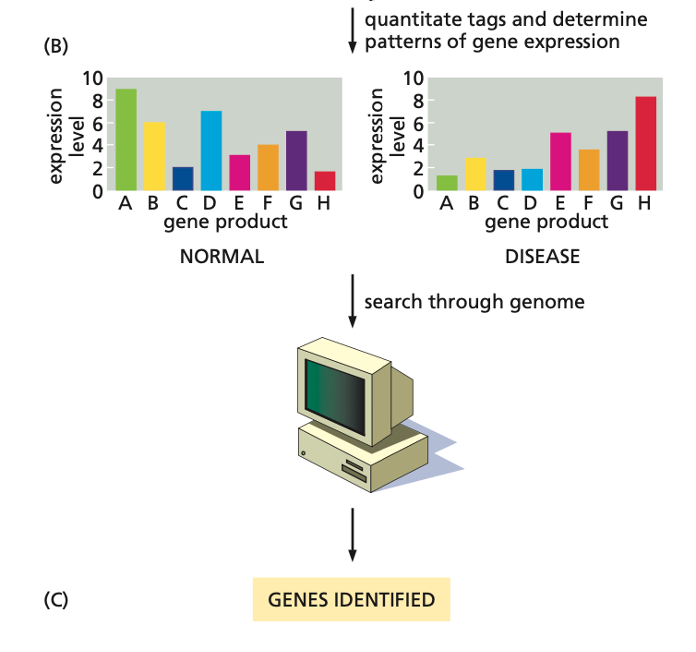
\includegraphics[width=0.9\textwidth]{SAGE2.png}
       \caption{}
       \label{fig:SAGE2}
    \end{subfigure}
    \caption{\emph{An outline of the SAGE method for comparing levels of gene expression. (A) Short sequence tags. The sequence tags are isolated and are linked together to produce long DNA molecules that can be cloned and sequenced. (B) Once sequenced, each tag can be calculated, resulting in a value that gives the expression level of the corresponding transcript~\cite{zvelebil_understanding_2008}.}}\label{fig:SAGE}
\end{figure}

A short sequence contains enough information to uniquely identify a gene. The sequence tags from the total cellular RNA can be linked together to form long DNA molecules. The total number of times a particular tag is observed the concatemers approximates the expression level of the corresponding gene. The data produced by SAGE include a list of the tags with their corresponding counts, providing a digital output of cellular gene expression.  Which allows the user to specify which organ is to be investigated. Libraries consisting of gene lists organized by the various types of tissues or cell lines are provided for further choice. The output from SAGE provides the SAGE tag, the UniGene ID, the gene description, and color and letter-coded differences in expression levels~\cite{zvelebil_understanding_2008}.


\subsubsection{Clustered gene expression data}

Clustered pattern data obtained from gene expression microarrays/genome bioinformatics can be used as a tool to identify new transcription factors or other cell-regulatory proteins. 

The clustered genes/proteins can be analyzed. Leading to a vast collection of data from many gene/protein expression experiments being available on the Web~\cite{zvelebil_understanding_2008}.

\clearpage
\subsubsection{Large Scale Protein Expression}

\begin{figure}[ht]
    \centering
    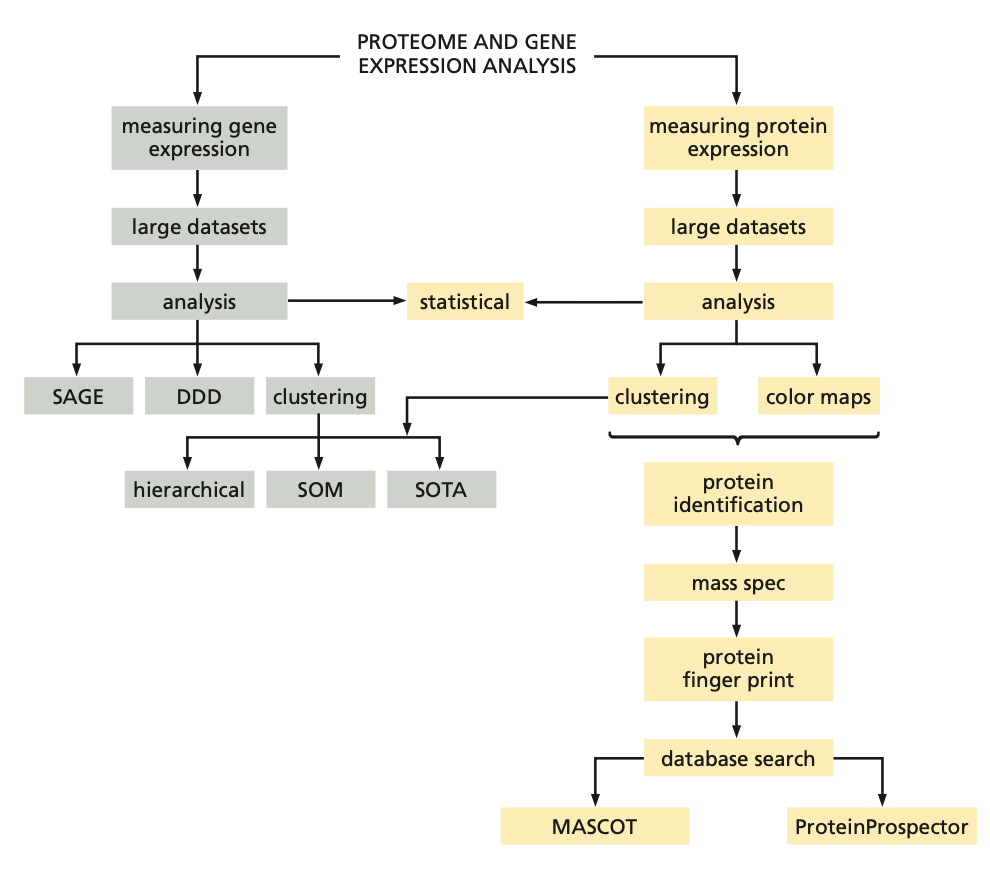
\includegraphics[width=0.5\textwidth]{Overlaping.png}
    \caption{\label{fig:Overlaping}Describing some experimental aspects of protein expression and of the analysis of the resulting data.~\cite{zvelebil_understanding_2008}.}
\end{figure}

For functional protein, mRNAs need to be translated, whilst the protein products can change which influence their function. For this reason we can measure and anlayse different proteins. 

There is more proteins than there are genes in a genome. Transcripts can be spliced in various ways to give different mRNAs, providing different protein products, from the same gene. However, proteins that can be modified after translation giving more different protien products.

Protien expressions can vary in a organism depending on the origin and it will also differ between the separate stages of an organism’s life cycle and under different environmental conditions~\cite{zvelebil_understanding_2008}.

\begin{definition}[proteome]
    The proteome refers to all the proteins that make up an organism at a specific point in time and under specific conditions.
\end{definition}

\clearpage

\subsubsection{RNAseq}

The transcriptome is important for revealing the molecular constituents of cells and tissues, interpreting the functional aspects of the genome, also for understanding development and disease~\cite{wang_rna-seq_2009}.

Many methods deduce and quantify the transcriptome, including hybridization or sequence-based approaches. For example, hybridization-based approaches involve incubating fluorescently labeled cDNA with microarrays or commercial high-density oligo microarrays~\cite{wang_rna-seq_2009}.

However, these methods have several limitations, such as: 
\begin{itemize}
    \item Dreliance upon existing knowledge about genome sequence.
    \item Limited dynamic range of detection owing to both background.
    \item High background levels owing to cross-hybridization~\cite{okoniewski_hybridization_2006}~\cite{royce_toward_2007}.
    \item saturation of signals.
\end{itemize}

\begin{definition}[transcriptome]
    The transcriptome is the complete set of transcripts in a cell, and their quantity, for a specific developmental stage or physiological condition. 
\end{definition}

Sequence-based approaches directly determine the cDNA sequence such as Tag-based methods which include SAGE, CAGE~\cite{kodzius_cage_2006}, MPSS~\cite{reinartz_massively_2002}.

Each approach is high throughput and can provide precise, gene expression levels. However, a significant portion of the short tags can not be uniquely mapped to the reference genome~\cite{wang_rna-seq_2009}.

RNA-Seq RNA sequencing has clear advantages over existing approaches it uses deep sequencing technologies where a population of RNA is converted to a library of cDNA fragments with adaptors attached to one or both ends. Each molecule is then sequenced in a high-throughput manner to obtain short sequences from one or both ends~\cite{wang_rna-seq_2009}.

\clearpage

\subsubsection{Bioinformatic Difficulties with Predictions on Proteins}

It is difficult to define the precise ends of the helices(The secondary structure of proteins is made up of a-helices and b-strands) for structures found in globular proteins that are not perfectly regular. Making it one step more difficult when trying to predict these structures~\cite{zvelebil_understanding_2008}.

To Note:
\begin{itemize}
    \item Several different types of b-sheet are found in protein structures.
    \item Turns, hairpins, and loops connect helices and strands. 
    \item Any chain between two regular structures is referred to as a loop.
    \item Mostly a loop will contain a turn (or even several).
\end{itemize} 

In antibody recognition, immunoglobulins employ loops at the edge of a b-sheet. All immunoglobulin structures with the same overall chain fold, but it is the difference at these loops that results in different results. Loops take up one of a limited number of structures called canonical forms. This type of classification is another reason why trying to predict both the structure and function of the protein is difficult~\cite{zvelebil_understanding_2008}.

\begin{definition}[Immunoglobulin]
    Immunoglobulins are heterodimeric proteins composed of two heavy and two light chains. Types of white blood cells that helps the body fight infection~\cite{schroeder_structure_2010}.
\end{definition}

\clearpage

\subsubsection{Alpha Fold}

AlphaFolds' goal is to predict the 3D coordinates of all heavy atoms for a given protein using the primary amino acid sequence and aligned sequences of homologues as inputs~\cite{jumper_highly_2021}.

Mutations in proteins can lead to misfolding which is often associated with disease states, for example, Alzheimer’s and Parkinson’s which is one of the challenges for alphaFold~\cite{felix_brief_nodate}.

The output is a file containing the 3D coordinates for every non-hydrogen atom in the protein. whilst showing the confidence levels for every amino acid residue, providing the reliability of the predicted structure~\cite{felix_brief_nodate}.

\subsubsection{Bioinformatics with Alpha Fold}

In July 2021, AlphaFold was developed by DeepMind and was made available to
the public~\cite{tunyasuvunakool_highly_2021}. 

Where it tries to solve the issue of invariant protein structures that are under translations and rotations~\cite{baldi_principled_nodate}.

AlphaFold is trained on protein chains from the PDB using the input sequence to query databases of protein sequences to generate a multiple sequence alignment~\cite{jumper_highly_2021}. Although we still do not exactly know how a protein sequence folds and alpha fold do not help in figuring this out its impact will likely be in accelerating and improving the production of new medications~\cite{nussinov_alphafold_2022}.


\subsubsection{AlphaFold 2}

The CASP14 was recently held which is a blind trial that critically assesses
techniques for protein structure prediction~\cite{david_alphafold_2022}, AlphaFold2 was entered and out-performed all competitors. 

Recently, RoseTTAFold was developed, trying to implement similar principles. Since then, other end-to-end structure predictors have emerged using different principles such as fast multiple sequence alignment processing in DMPFold218 and language model representations.\cite{bryant_improved_2022}.

We use the root mean square deviation, to calculate the similarity between the two structures, AlphaFold models had an accuracy of 0.96 compared to 2.80 which was the second-best score. AlphaFold models also had a high level of accuracy in predicting the position of residue side chains when the protein backbone prediction was accurate~\cite{david_alphafold_2022}~\cite{jumper_highly_2021}.

\clearpage

\subsection{The Protein Data Bank and the File Formats}

\subsubsection{Protein Data Bank}

The Protein Data Bank was established at Brookhaven National Laboratories ~\cite{bernstein_protein_1977} in 1971 as an archive for biological macromolecular crystal structures~\cite{berman_protein_2000}.

\begin{definition}[Macromolecular]
    Macromolecular is any very large molecule, usually with a diameter ranging from about 100 to 10,000 angstroms
\end{definition}

It is an information source for data retrieved from atomic structures, crystallography, and three-dimensional structures of biomolecules, including nucleic acids and proteins~\cite{behzadi_worldwide_2021}. 

At the time this was the first open-access digital data resource in biology which started with just seven protein structures~\cite{burley_rcsb_2022}.

Various groups such as the Protein Data Bank in Europe, Protein Data Bank Japan help manage the Protein Data Bank archive. Current wwPDB members also include the ElectronMicroscopy Data Bank and the Biological Magnetic Resonance Bank~\cite{burley_rcsb_2022}.

Protein Data Bank China has recently joined the wwPDB as an Associate Member with its role as wwPDBdesignated PDB Archive Keeper. Where they are responsible for weekly updates of the archive and safeguarding both digital information and a physical archive of correspondence~\cite{burley1_rcsb_2022}.

The management of PDB must comply with FAIR (the acronym depicts: Findable, Accessible, Interoperable, Reusable) and FACT~\cite{van_der_aalst_responsible_2017} guiding principles for scientific data~\cite{wilkinson_fair_2016}~\cite{westbrook_impact_2020}.

\begin{table}[h!]
    \begin{center}
    \label{tab:FAIR}
        \begin{tabular}{c|p{0.65\linewidth}}
        The FAIR Guiding Principles\\
        \hline
        \\
        To be Findable: & F1. (meta)data are assigned a globally unique and persistent identifier\\
        & F2. data are described with rich metadata (defined by R1 below)\\ & F3. metadata clearly and explicitly include the identifier of the data it describes\\ & F4. (meta)data are registered or indexed in a searchable resource\\
        \\
        \hline
        \\
        To be Accessible: & A1. (meta)data are retrievable by their identifier using a standardized communications protoco\\
        & A1.1 the protocol is open, free, and universally implementable\\ & A1.2 the protocol allows for an authentication and authorization procedure, where necessary\\ & A2. metadata are accessible, even when the data are no longer available
        \\
        \hline
        \\
        To be Interoperable: & I1. (meta)data use a formal, accessible, shared, and broadly applicable language for knowledge representation.\\
        & I2. (meta)data use vocabularies that follow FAIR principles\\ & I3. (meta)data include qualified references to other (meta)data\\
        \\
        \hline
        \\
        To be Reusable: & R1. meta(data) are richly described with a plurality of accurate and relevant attributes\\
        & R1.1. (meta)data are released with a clear and accessible data usage license\\ & R1.2. (meta)data are associated with detailed provenance\\ &
        R1.3. (meta)data meet domain-relevant community standards\\
        \end{tabular}
        \caption{\label{Fair}The guidlines to what builds up the FAIR principles~\cite{wilkinson_fair_2016}}
    \end{center}
\end{table}

\clearpage

\subsubsection{Aims and Objectives of PDB}

Enzymology, electron microscopy, computational chemistry small molecule crystallography, biochemistry, biophysics, macromolecular crystallography and nuclear magnetic resonance spectrometry all help the aims and goals of the PDB archive~\cite{behzadi_worldwide_2021}.

\begin{definition}[Enzymology]
    Enzymology is the branch of biochemistry aiming to understand how enzymes work
\end{definition}

\begin{definition}[Electron Microscopy]
    Electron microscopy is a technique for obtaining high resolution images of biological and non-biological specimens.
\end{definition}

PDBs provide open access to nearly 200 000 archived, validated, and biocurated experimentally determined three-dimensional structures of biological macromolecules.3D structures archived in the PDB have enabled important scientific breakthroughs by basic and applied researchers~\cite{burley_impact_2021}. Open access to PDB data without restrictions on usage has also aided structural bioinformatics in areas such as computational biology.

\clearpage

\subsubsection{Recent Project}

A project was undertaken to change the information management services for RCSB.org. The idea was to have developed a primary place for studying 3D biostructures by extending RCSB.org web portal functionality to support parallel delivery of more than one million CSMs publicly available from AlphaFold DB and ModelArchive together~\cite{burley1_rcsb_2022}.

\subsubsection{Covid}

During the COVID-19 pandemic, more than 2000 structures associated with the agent of the coronavirus disease were released and have become accessible to global users for free. The properties of these structures give us this opportunity to find out the ligand binding sites, the spatial conformation of ligands, protein-to-protein interactions, and amino acid substitutions regarding different viral proteins. Moreover, chemical, functional and energetic characteristics can also be gained to describe the potential capabilities of each molecule. These properties might aid us to determine the potential drug targets for drug design and vaccine preparation~\cite{lubin_evolution_2020}.

\subsubsection{PDB Currently}

As of 2022, the PDB has a vast number of 3D biostructures, eukaryotic protein structures exceeded 105 000. Bacterial protein structures were also numerous, totaling nearly 66 000. Archaeal protein structures were the least numerous totaling 5500. However the PDB coverage is decidedly limited, with mouse protein structures being most numerous at 8000 structures~\cite{burley_open-access_2021}. 

We have powerful tools developed by RCSB PDB for searching and analysis which include structure, sequence, sequence motif, structure motif, and visualization~\cite{burley1_rcsb_2022}.

Upon reaching the RCSB.org home page, users can query, organize, visualize, analyse, compare, and explore PDB structures and CSMs side-by-side. Searching 3D structure information can encompass PDB structures and CSMs or be limited to PDB structures only. Either PDB structures or CSMs can be excluded from the search results. The two types of structure information accessible via RCSB.org are clearly distinguished from each other. Top bar searching and data delivery for PDB structures and CSMs~\cite{burley1_rcsb_2022}.

\begin{figure}[ht]
    \centering
    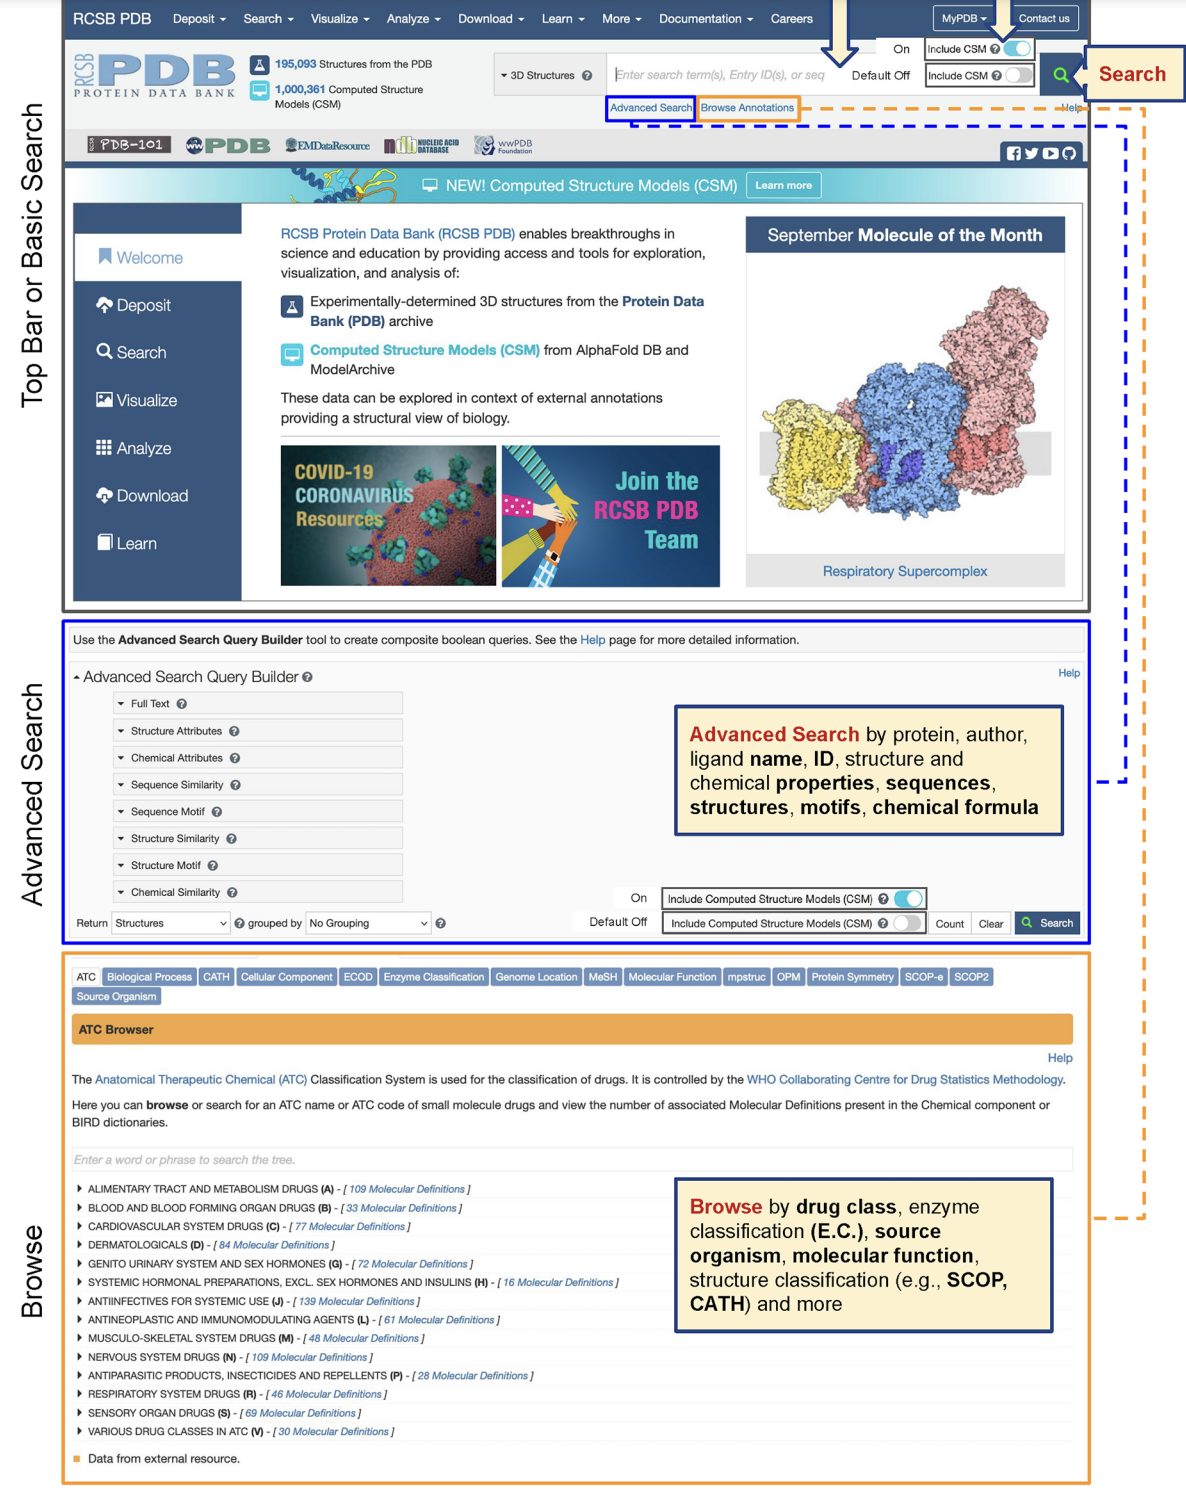
\includegraphics[width=0.5\textwidth]{PDB Site.png}
    \caption{\label{fig:PDB}Search options at RCSB.org include Top Bar or Basic Search; Advanced Search; and Browse Annotations~\cite{burley1_rcsb_2022}.}
\end{figure}

\begin{figure}[!ht]
    \centering
    \begin{subfigure}[t]{.45\textwidth}
        \centering
        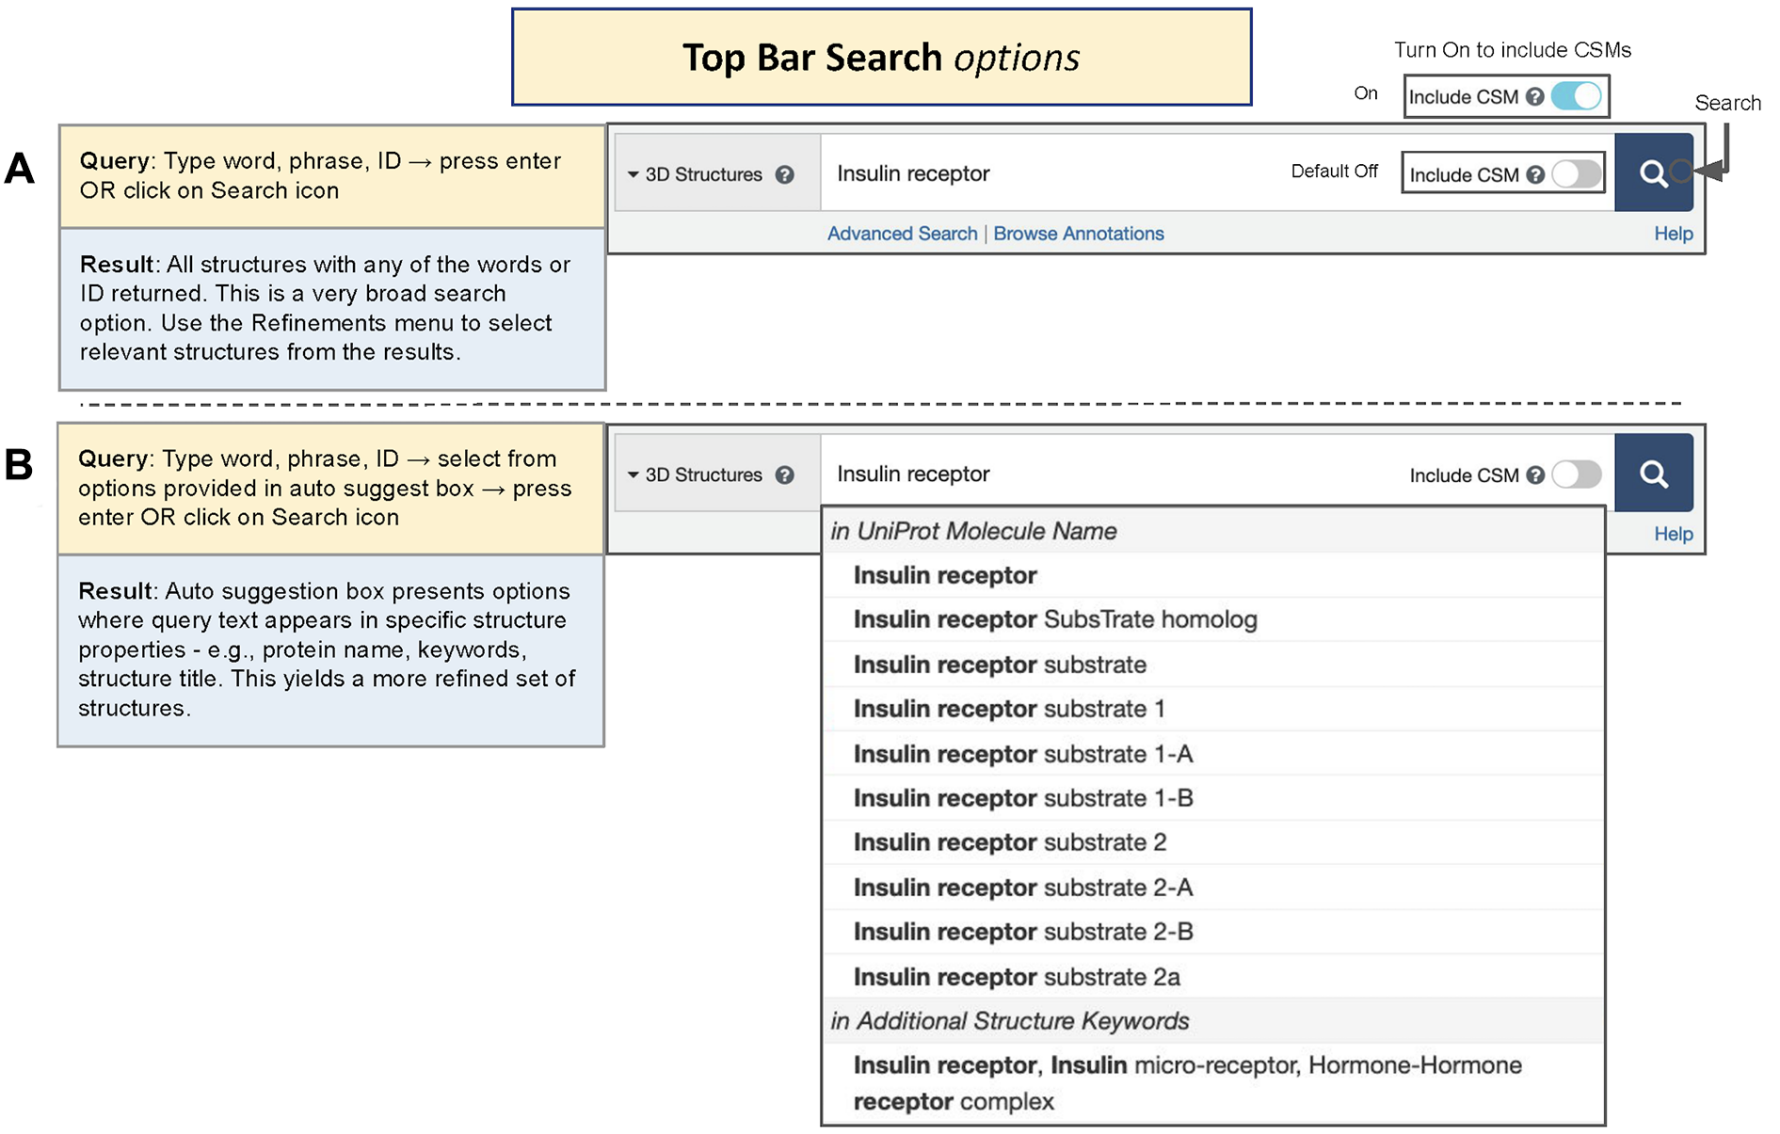
\includegraphics[width=0.9\textwidth]{Top Bar Search A.png}
        \label{fig:Top1} 
    \end{subfigure}
    \begin{subfigure}[t]{.45\textwidth}
       \centering
       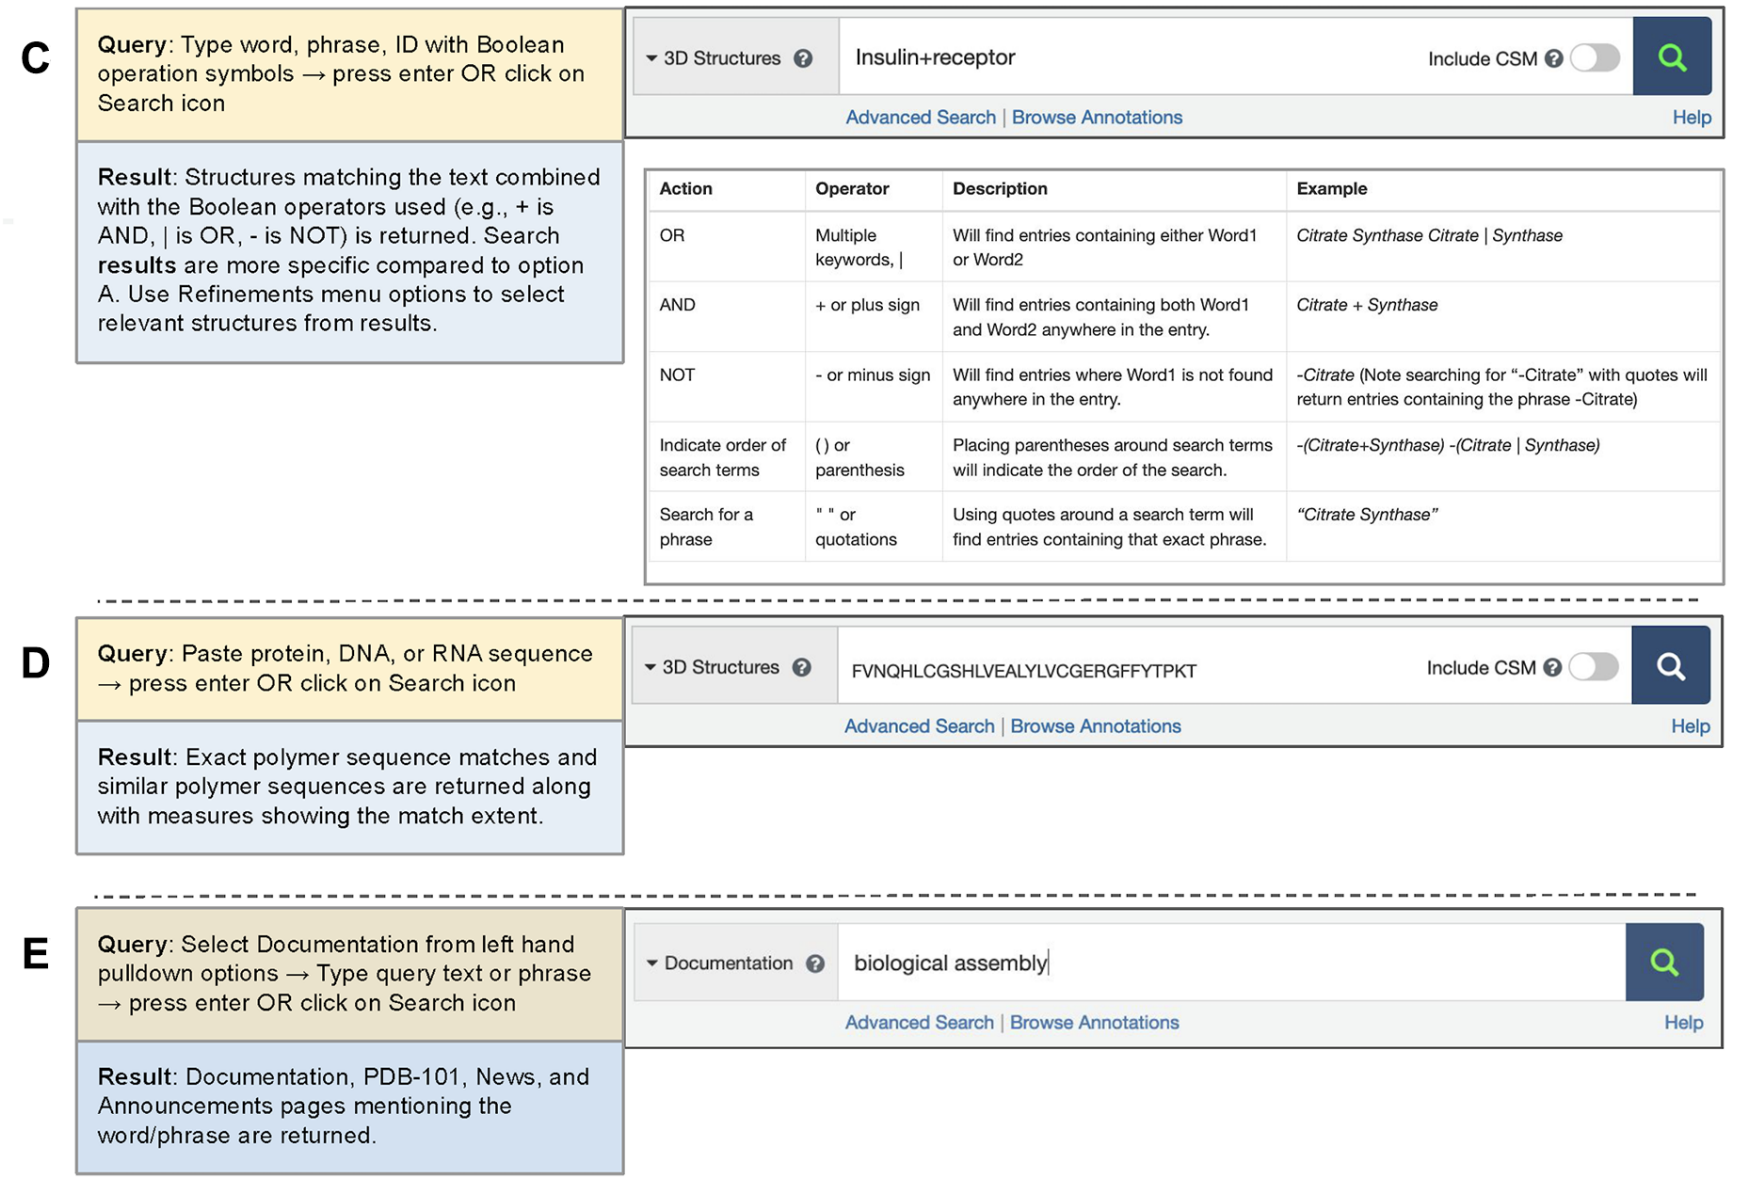
\includegraphics[width=0.9\textwidth]{Top Bar Search B.png}
       \label{fig:Top2}
    \end{subfigure}
    \caption{\emph{Top Bar or Basic Search options available from every RCSB.org web page. Examples of searching for 3D structures using (A) simple text string insulin receptor; (B) drop down autosuggestions based on the text string insulin receptor; (C) Boolean operators to combine insulin + receptor (+ = AND); or (D) an amino acid sequence. (E) Searching RCSB.org documentation using a text string biological assembly~\cite{burley1_rcsb_2022}}}
\end{figure}
\clearpage

\subsubsection{Recent RCSB PDB data architecture improvements}

In 2020, RCSB PDB had an upgrade of its delivery architecture~\cite{rose_rcsb_2021}at RCSB.org~\cite{powerful_rcsb_2021}. 

The legacy monolithic data delivery application was changed into a distributed deployment of individual microservices, each with a single responsibility. 

Data access services provide both Representational State Transfer and GraphQL API access to a data warehouse hosted in a MongoDB documentoriented database. Originally, advanced Search QueryBuilder functionality encompassed text, PDB data attributes, 3D structure, sequence, biopolymer sequence motif, and chemical similarity. Every search function is implemented as an independent service.

A separate search service is responsible for launching each search function, combining and delivering their integrated results to public programmatic search APIs. When each service has a single responsibility, we have greater flexibility in scaling the deployment of services in response to changes in user load and significant reductions in the time required to develop, test, and deploy new features. The Sequence Motif search function has been extended with a new 3D Structure Motifsearch capability~\cite{bittrich_real-time_2020}. 

\subsubsection{Recent advances in RCSB PDB data integration}

RCSB PDB integrates the content of each expertly biocurated Entry with information from more than 50 external data resources. 

Integrated external data needs to follow a data schema that defines the organization of the RCSB PDB data warehouse. Finally, it is available to RCSB PDB front-end services, public data access APIs, and our text search indexing service~\cite{burley_rcsb_2022}.

\begin{table}[h!]
    \begin{center}
    \label{tab:External Data}
        \begin{tabular}{c|p{0.58\linewidth}}
        External Resources\\
        \hline
        \\
        AlphaFold DB & Computed Structure Models by AlphaFold2
        \\
        \hline
        \\
        ATC & 	Anatomical Therapeutic Chemical (ATC) Classification System from World Health Organization
        \\
        \hline
        \\
        Binding MOAD & Binding affinities
        \\
        \hline
        \\
        Binding DB & Binding affinities
        \\
        \hline
        \\
        BMRB & BMRB-to-PDB mappings
        \\
        \hline
        \\
        Cambridge structural Database & Crystallographic small molecule data from the Cambridge Crystallographic Data Centre
        \\
        \hline
        \\
        CATH & 	Protein structure classification- Class, Architecture, Topology/fold, and Homologous superfamily    
        \\
        \hline
        \\
        ChEMBL & Manually curated database of bioactive molecules with drug-like properties
        \\
        \hline
        \\
        CSD & Cambridge Structural Database: Validated and curated small-molecule organic and metal-organic crystal structures from the Cambridge Crystallographic Data Centre
        \\
        \hline
        \\
        DrugBank & Drug and drug target data
        \\
        \hline
        \\
        ECOD & Evolutionary Classification of Protein Domains
        \\
        \hline
        \\
        EMDB & 3DEM density maps and associated metadata
        \\
        \hline
        \\
        ExplorEnz & IUBMB Enzyme nomenclature and classification
        \\
        \hline
        \\
        Gencode & Human and Mouse Gene annotations
        \end{tabular}
        \caption{\label{External Data}Some of the External Resources Integrated Into RCSB PDB}
    \end{center}
\end{table}


\subsubsection{Recent PDBx/mmCIF data standard improvements}

The PDBx/mmCIF data standard is maintained by the wwPDB organization in collaboration with wwPDBPDBx/mmCIF Working Group domain experts recruited from the scientific community. The PDBx/mmCIF web resource supports browse and search access to standard terminology. The Working Group includes developers for many of the widely used structure determination software systems, who ensure that data produced by these programs comply with the PDBx/mmCIF data standard, generating complete and correct data files for PDB deposition. The wwPDB and the Working Group collaborate on developing terminologies for new and rapidly evolving methodologies such as Free Electron Laser, 3DEM, Serial Crystallography, and X-ray, whilst improving representations for existing data content. Most recently, the Working Group has focused on modernizing content descriptions for processed X-ray diffraction data, including extensions describing anisotropic diffraction limits, unmerged reflection data, and new quality metrics of anomalous diffraction data. Deposition and delivery improve our ability to assess experimental data quality, and every PDB data consumer's ability to Find and Reuse relevant PDB Entries~\cite{burley_rcsb_2022}.

\clearpage

\subsubsection{Future and struggles of PDB}
\subsubsection{Future}
As the PDB archive has started its 52nd year, it gives open access to analyses of structures and much more to: basic and applied researchers, educators, and students spanning fundamental biology, biomedicine, bioenergy, bioengineering, and biotechnology, with key points that help many communities that use this facility. Firstly It delivers Data In and Data Out services efficiently to a user base that is now numbering many millions worldwide. Secondly, it has wwPDB partners that process, validate, and biocurate the growing number of increasingly complex PDB depositions received. Manages and safeguards the growing PDB archive in its role as wwPDB designated Archive Keeper. Thirdly it enables searching, visualization, exploration, and analysis of experimentally-determined PDB structures integrated with more than one million CSMs through its web portal.~\cite{burley1_rcsb_2022}.

\subsubsection{Struggles}
Even after all the advancments PDB has gone through there are still additional challenges lying ahead which include:

\begin{itemize}
    \item Rapid growth in public-domain CSMs of individual polypeptide chains, already numbering >200 million at the time of writing.
    \item Anticipated advances in AI/ML-based prediction of structures of multi-protein complexes.
    \item Continued development of biomolecular structure determination methods using X-ray Free Electron Lasers, revealing the microscopic details of chemical reactions in real time.
    \item Growth in the number and complexity of atomic-level cryoelectrontomography structures of macromolecular machines.
    \item Integration of PDB structures and CSMs with complementary information coming from correlative light microscopy and related imaging methods across length scales ranging from atoms to small molecules to individual biomolecules to macromolecular assemblies to organelles to cells and ultimately tissues
    \item Merging of the PDB-Dev prototype archiving system for integrative methods structures with the PDB archive
    \item Federating other biodata resources, such as the SmallAngle Scattering Database and the Proteomics Identification Database, with the PDB, EMDB and BMRB core archives jointly managed by the wwPDB partnership
\end{itemize}
~\cite{burley1_rcsb_2022}.

\clearpage

\subsubsection{File Formats}

The PDB archive holds a few different types of file types that hold data such as atomic coordinates and other information describing proteins and other biological macromolecules. Depending on what the data is created from it can fall into a different category.

\subsubsection{PDB Data}

The main information in the PDB archive is coordinate files for biological molecules. These files list the atoms in each protein and their 3D coordinates.

These files are available in several formats:

\begin{itemize}
    \item PDB
    \item mmCIF
    \item XML
\end{itemize}

The header section of the text summarizes the protein, citation information, and the details of the structure solution, which is then followed by the sequence and a long list of the atoms and their coordinates. It also contains the experimental observations used to determine atomic coordinates~\cite{noauthor_pdb101_nodate}.

\clearpage

\subsubsection{.pdb Files}

The PB format consists of a collection of records that describe the atomic coordinates, chemical and biochemical features, and experimental details of the structure determination~\cite{westbrook_pdb_2003}.

Each item of data in the PDB format is assigned to a one of PDB record types (HEADER. SOURCE. REMARK, etc.). The ATOM records the atomic coordinate data~\cite{westbrook_pdb_2003}.

PDB format has been extended with new REMARK records. For example, REMARK 3 that encodes refinement information has been modified and extended for each new refinement program and program version~\cite{westbrook_pdb_2003}.

The PB format uses fixed-width fields to represent data, so we have limits on the size of certain items of data. For example, we cant have more then 99,999 atoms and polymer chain can be only one character. This means some structures are devided into multiple files~\cite{westbrook_pdb_2003}.

\begin{figure}[ht]
    \centering
    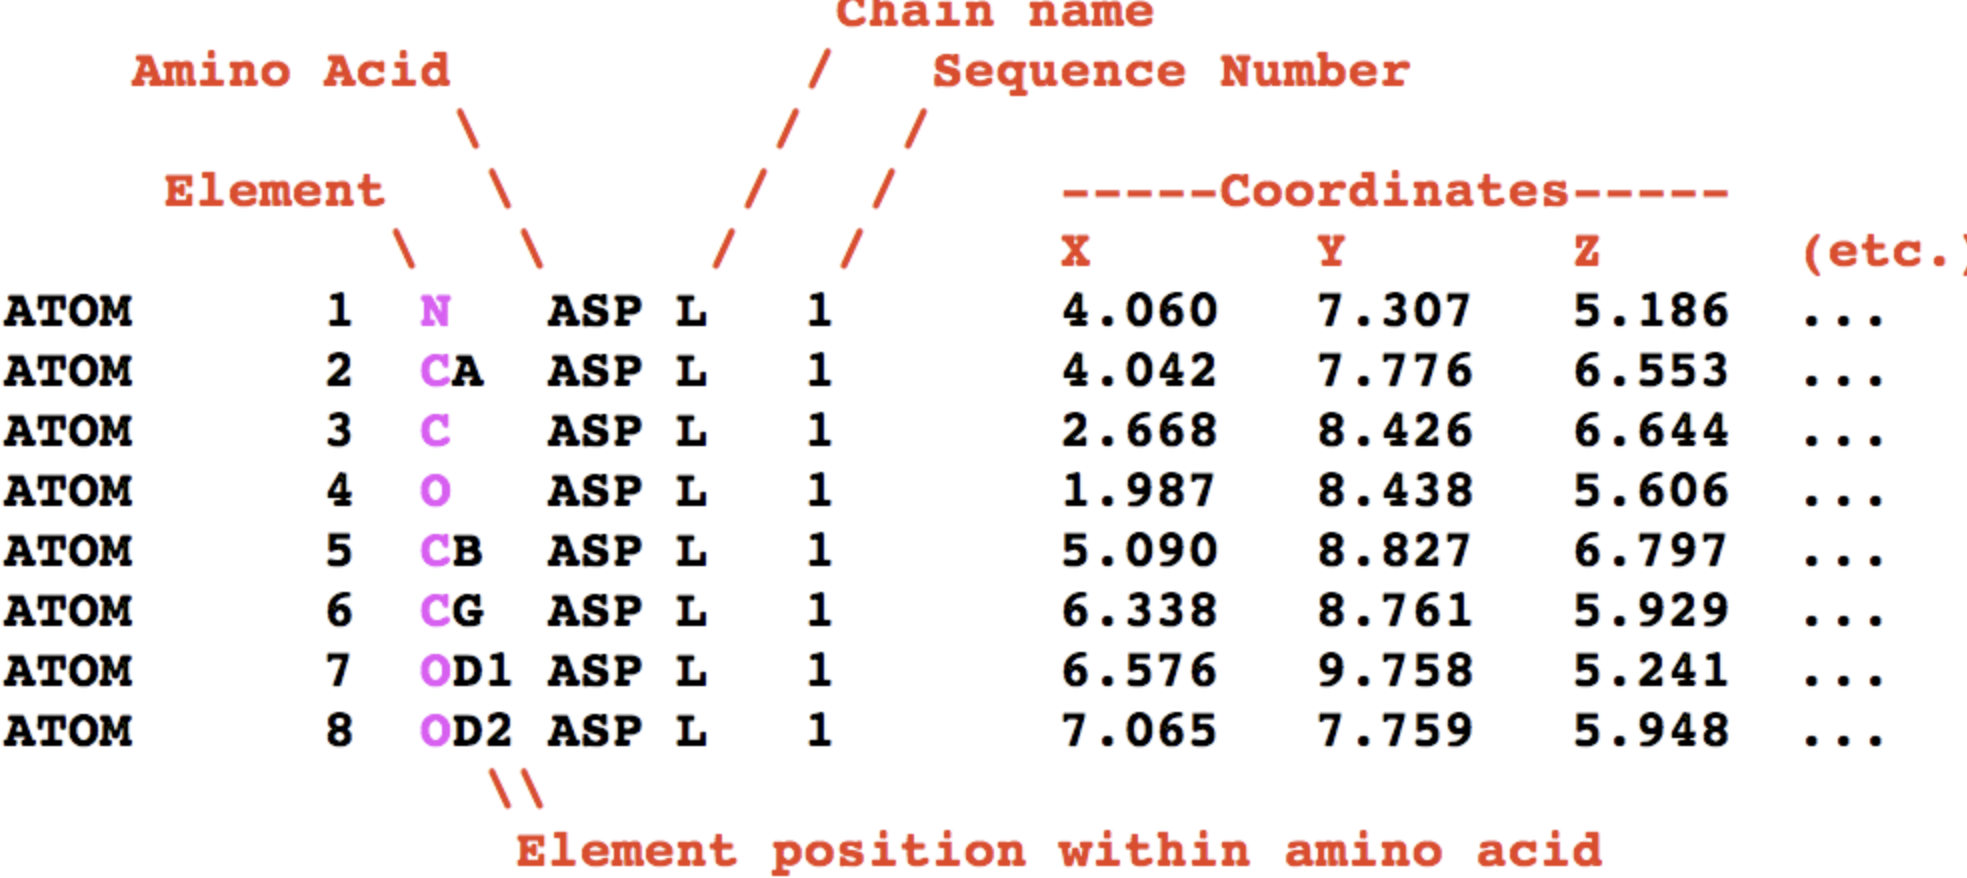
\includegraphics[width=0.5\textwidth]{PDB File.png}
    \caption{\label{fig:PDB file}Showing contents of a PDB file for the Atom values~\cite{adams_announcing_2019}.}
\end{figure}

\clearpage

\subsubsection{.mmCIF Files}
Mmcif is a dictionary-based approach to data extracted from crystallographic experiments~\cite{westbrook_pdb_2003}.

It includes all the data we can find in a pdb file. Also, we have sufficient data names so that the experimental section of a structure paper can be written automatically and to facilitate the development of tools i.e. computer programs could easily access and validate mmCIF data files~\cite{westbrook_pdb_2003}.

\subsubsection{.xml}

XML builds from a PDB Exchange dictionary. Although presented in very different syntaxes, the PDB Exchange and XML representations use the same logical data organization.~\cite{westbrook_pdbml_2005}.

The dictionary data block is mapped to the standard top-level XML schema element, and the data file data block is mapped to a datablock element. Category or table definitions in the Exchange dictionary are described as XML complex types. The category definition.~\cite{westbrook_pdbml_2005}.

\vspace{70px}

\begin{figure}[ht]
    \centering
    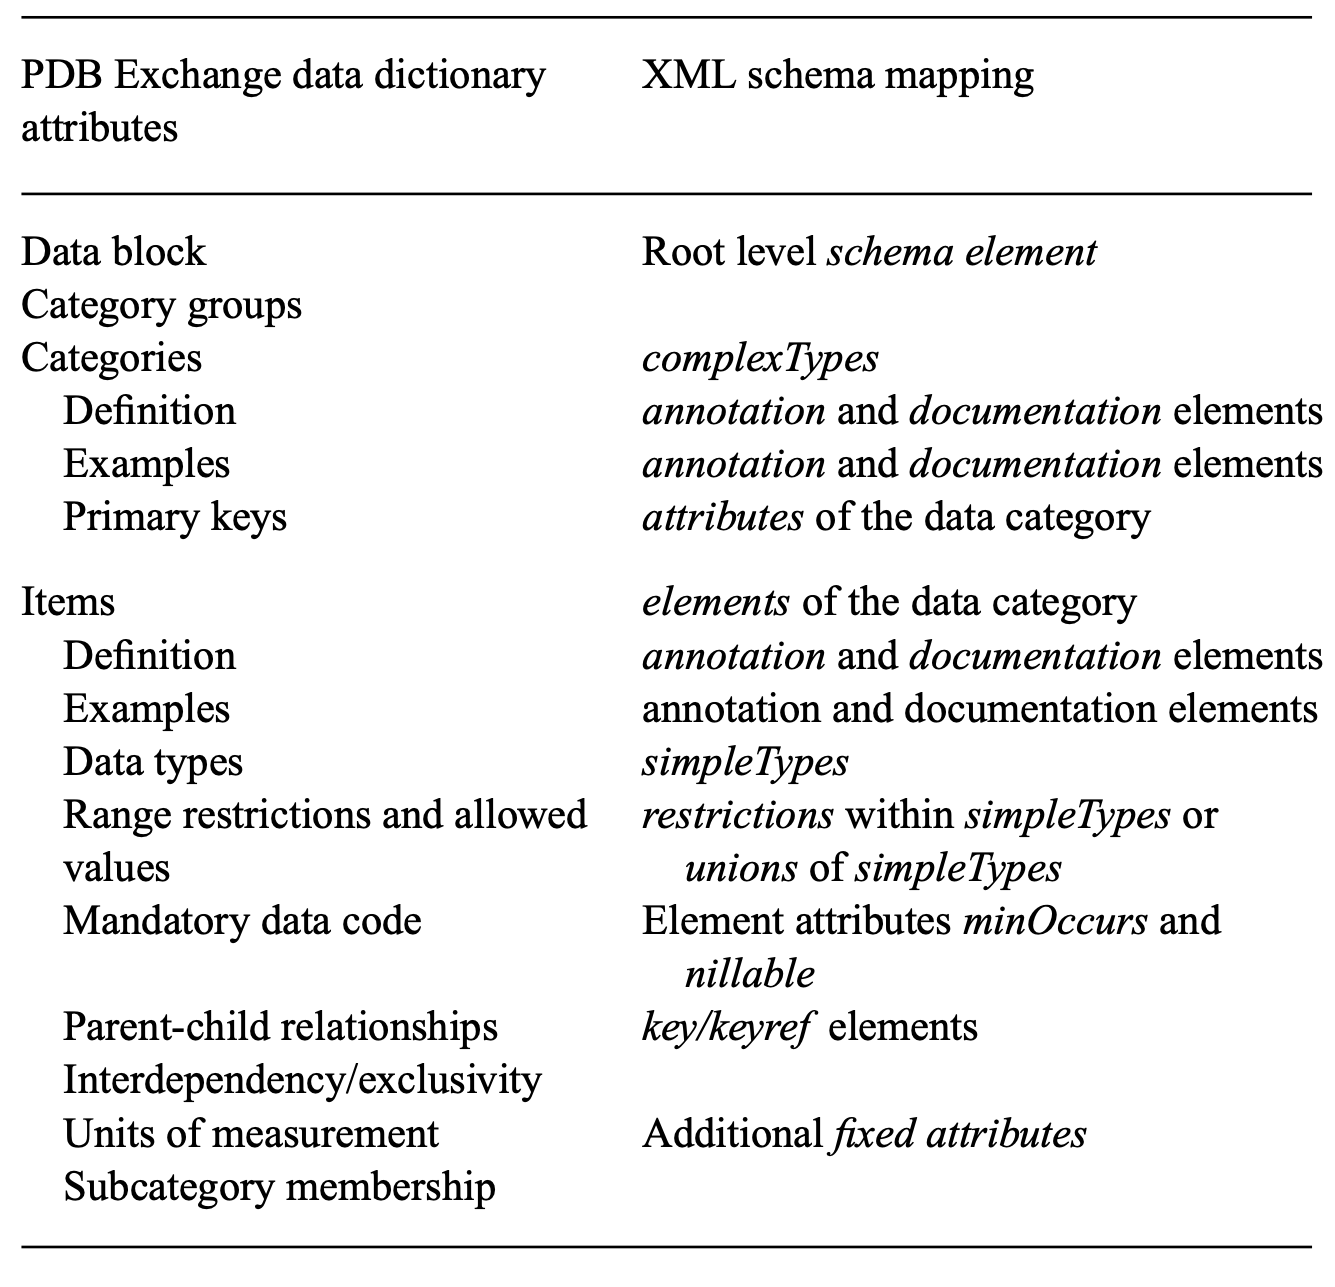
\includegraphics[width=0.5\textwidth]{xml.png}
    \caption{\label{fig:xml}Summary of the correspondences between PDB Exchange data dictionary and XML schema metadata~\cite{westbrook_pdbml_2005}.}
\end{figure}

\clearpage

\subsubsection{Visualizing Structures}

PDB files can be viewed from text editors but we can also use a browsing or visualization program. RCSB PDB allows you to search and explore the information, including information on experimental methods and the chemistry and biology of the protein. Visualization programs allow to read of the PDB file and, display the protein structure generating custom pictures of it. These programs can contain analysis tools that allow you to measure distances and bond angles, and identify interesting structural features~\cite{noauthor_pdb101_nodate}.

\subsubsection{Reading Coordinate Files}

Before exploring structures in the PDB archive we need some prior understanding of the coordinate files. For example, we can find a diverse mixture of biological molecules, small molecules, ions, and water which can get confusing we can use the names and chain IDs to help sort these out. In structures determined from crystallography, atoms are annotated with temperature factors that describe their vibration and occupancies that show if they are seen in several conformations. NMR structures often include several different models of the molecule~\cite{noauthor_pdb101_nodate}.

\subsubsection{Potential Challanges}

There are some things to note as you could fall into some challenges when browsing through the PDB archive. Many structures, particularly those determined by crystallography, only include information about part of the functional biological assembly. One thing to note is that the PDB can aid with this. Another note is many PDB entries are missing portions of the molecule that were not observed in the experiment. These include structures that include only alpha carbon positions, structures with missing loops, structures of individual domains, or subunits from a larger molecule. In addition, most of the crystallographic structure entries do not have information on hydrogen atoms~\cite{noauthor_pdb101_nodate}.

\clearpage

\subsection{Hadoop spark and pyspark}

\subsubsection{What is Hadoop}

Hadoop is an open-source framework for writing and running distributed applications that process large amounts of data.  Key aspects making it valuable such 1. Accessible 2.Robust 3. Scalable 4.simple~\cite{lam_hadoop_2010}.

HDFS is used in haddop which is a filessystem and a MapReduce engine. With one master node and many worker nodes. The master node provides instructions to the worker nodes and computations are performed on the worker nodes.~\cite{hazarika_performance_2017}.

\subsubsection{Mapper}
Input key/value pairs are mapped to a set of key/value pairs. The mapper then sorts the key-value pairs by the keys. Partitioners are mainly responsible for providing intermediate key/values to the reducers~\cite{patel_addressing_2012}~\cite{hazarika_performance_2017}.

\subsubsection{Reducer}

Firstly, the reducer combines data having the same key from different map functions. The values having the same key are reduced to a smaller set of values and output is produced~\cite{hazarika_performance_2017}.

\clearpage

\subsubsection{What is Spark}
Apache Spark is a popular open-source platform for large-scale data processing used for iterative machine learning tasks~\cite{meng_mllib_2016}.

Spark is a cluster computing system providing APIs in Java, Scala, Python (pySpark), and R, along with an optimized engine that supports general execution graphs. Moreover, Spark is efficient at iterative computations so it is suited for the development of large-scale machine learning applications~\cite{meng_mllib_2016}.

Spark is a quick and general engine used for analysing large-scale data stored across a cluster of computers. Spark uses in-memory cluster computing which is its most important feature for increasing the processing speed of an application. It combines SQL streaming and complex analytics~\cite{hazarika_performance_2017}.

\subsubsection{Spark Architecture}

There are five core components that make Spark so powerful and easy to use. The core architecture of Spark consists of the following layers:

\begin{itemize}
    \item Storage
    \item Resource management
    \item Engine
    \item Ecosystem
    \item APIs
\end{itemize}
~\cite{singh_manage_2022}.

\subsubsection{Storage}
Before using Spark, data must be made available in order to process it. This data can reside in any kind of database. Spark offers multiple options to use different categories of data sources, to be able to process it on a large scale. Spark allows you to use traditional relational databases as well as NoSQL, such as Cassandra and MongoDB~\cite{singh_manage_2022}.
\clearpage

\subsubsection{Resource Management}
The next layer consists of a resource manager. As Spark works on a set of machines (it also can work on a single machine with multiple cores), it is known as a Spark cluster. Typically, there is a resource manager in any cluster that efficiently handles the workload between these resources. The two most widely used resource managers are YARN and Mesos. The resource manager has two main components internally~\cite{singh_manage_2022}:

\begin{itemize}
    \item Cluster manager
    \item Worker
\end{itemize}

It’s kind of like master-slave architecture, in which the cluster manager acts as a master node, and the worker acts as a slave node in the cluster. The cluster manager keeps track of all information pertaining to the worker nodes and their current status. Cluster managers always maintain the following information~\cite{singh_manage_2022}:

\begin{itemize}
    \item Status of worker node (busy/available)
    \item Location of worker node
    \item Memory of worker node
    \item Total CPU cores of worker node
\end{itemize}

The main role of the cluster manager is to manage the worker nodes and assign them tasks, based on the availability and capacity of the worker node. On the other hand, a worker node is only responsible for executing the task it’s given by the cluster manager~\cite{singh_manage_2022}.

The tasks that are given to the worker nodes are generally the individual pieces of the overall Spark application. The Spark application contains two parts~\cite{singh_manage_2022}:

\begin{itemize}
    \item Task
    \item Spark driver
\end{itemize}

The task is the data processing logic that has been written in either PySpark or Spark R code. It can be as simple as taking a total frequency count of words to a very complex set of instructions on an unstructured dataset. The second component is Spark driver, the main controller of a Spark application, which consistently interacts with a cluster manager to find out which worker nodes can be used to execute the request. The role of the Spark driver is to request the cluster manager to initiate the Spark executor for every worker node~\cite{singh_manage_2022}.

\clearpage

\subsubsection{Engine and Ecosystem}

The base of the Spark architecture is its core, which is built on top of RDDs (Resilient Distributed Datasets) and offers multiple APIs for building other libraries and ecosystems by Spark contributors. It contains two parts: the distributed computing infrastructure and the RDD programming abstraction. The default libraries in the Spark toolkit come as four different offerings~\cite{singh_manage_2022}.

\subsubsection{Spark SQL}

SQL being used by most of the ETL operators across the globe makes it a logical choice to be part of Spark offerings. It allows Spark users to perform structured data processing by running SQL queries. In actuality, Spark SQL leverages the catalyst optimizer to perform the optimizations during the execution of SQL queries. Another advantage of using Spark SQL is that it can easily deal with multiple database files and storage systems such as SQL, NoSQL, Parquet, etc~\cite{singh_manage_2022}.

\subsubsection{MLlib}

Training machine learning models on big datasets was starting to become a huge challenge, until Spark’s MLlib (Machine Learning library) came into existence. MLlib gives you the ability to train machine learning models on
huge datasets, using Spark clusters. It allows you to build in supervised, unsupervised, and recommender systems; NLP-based models; and deep learning, as well as within the Spark ML library~\cite{singh_manage_2022}.


\subsubsection{Structured Streaming}

The Spark Streaming library provides the functionality to read and process real-time streaming data. The incoming data can be batch data or near real-time data from different sources. Structured Streaming is capable of ingesting real-time data from such sources as Flume, Kafka, Twitter, etc~\cite{singh_manage_2022}.

\subsubsection{Graph X}

This is a library that sits on top of the Spark core and allows users to process specific types of data (graph dataframes), which consists of nodes and edges. A typical graph is used to model the relationship between the different objects involved. The nodes represent the object, and the edge between the nodes represents the relationship between them. Graph dataframes are mainly used in network analysis, and Graph X makes it possible to have distributed processing of such graph dataframes~\cite{singh_manage_2022}.
\clearpage

\subsubsection{Programming Language APIs}

Spark is available in four languages. Because Spark is built using Scala, that becomes the native language. Apart from Scala, we can also use Python, Java, and R~\cite{singh_manage_2022}.

\subsubsection{Spark Execution}

Any Spark application spins off a single driver process (that can contain multiple jobs) on the master node that then directs executor processes (that contain multiple tasks) distributed to a number of worker nodes shown ~\ref{fig:Execute.png}.

\begin{figure}[ht]
    \centering
    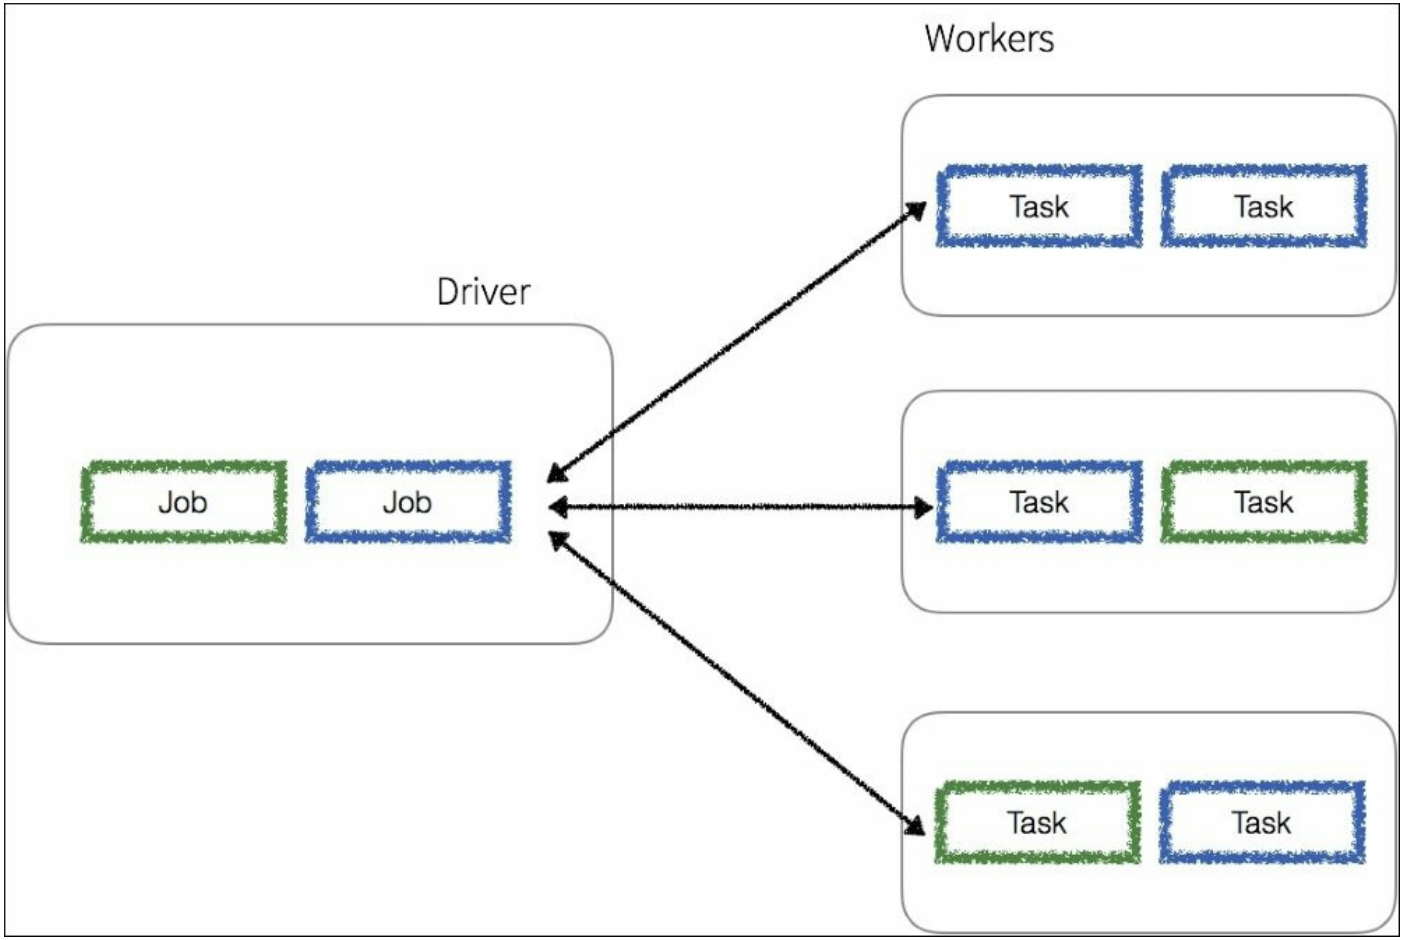
\includegraphics[width=0.5\textwidth]{Execute.png}
    \caption{\label{fig:Execute.png}Think of somthing to say~\cite{drabas_learning_2017}.}
\end{figure}


The driver process determines the number and the composition of the task processes directed to the executor nodes based on the graph generated for the given job. Note, that any worker node can execute tasks from a number of different jobs~\cite{drabas_learning_2017}.

\clearpage

\subsubsection{Spark vs Hadoop}

\begin{table}[ht!]
    \begin{center}
    \label{tab:Amino acids}
        \begin{tabular}{p{0.6\linewidth}|p{0.35\linewidth}}
        Hadoop Map Reduce & Spark\\
        \hline
        \\
        For Applications that repeatedly reuse the same set of data, map reduce is very inefficient. & Spark uses in-memory processing, reusing it for faster computation.
        \\
        \hline
        \\
        MapReduce is quite faster in batch processing. & As memory size is limited, it would be quite slower in batch processing of huge data set.
        \\
        \hline
        \\
        Data is stored in disk for processing. & Data is stored in main memory. As it is an inmemory computation engine entire data is copied. 
        \\
        \hline
        \\
        Difficulty in processing and modifying data in real time due to its high latency. & Used to process and modify data in real time due to its low latency. 
        \\
        \hline
        \\
        Predominantly used to process from bygone datasets. & Predominantly used for streaming, batch processing and machine learning
        \\
        \hline
        \\
        For fault tolerance, MapReduce uses replication. & For fault tolerance, Spark uses RDDs.
        \\
        \hline
        \\
        It merges and partitions shuffle files. & It does not merges and partition shuffle files. 
        \\
        \hline
        \\
        Primarily disk based computation. & Primarily RAM based computation.
        \\
        \end{tabular}
        \caption{\label{hadoopvsspark}Showing the differences between haddop and spark~\cite{hazarika_performance_2017}.}
    \end{center}
\end{table}

\clearpage

\begin{table}[ht!]
    \begin{center}
    \label{tab:Amino acids}
        \begin{tabular}{c|cc}
        Number of words & Hadoop (Sec) & Spark(Sec)\\
        \hline
        \\
        100 & 79 & 28.841
        \\
        1000 & 91 & 31.185
        \\
        10000 & 96 & 35.181
        \\
        100000 & 103 & 36.969
        \\
        1000000 & 116 & 39.569
        \end{tabular}
        \caption{\label{Results1}Comparision of Execution time for wordcount program~\cite{hazarika_performance_2017}.}
    \end{center}
\end{table}

\begin{table}[ht!]
    \begin{center}
    \label{tab:Amino acids}
        \begin{tabular}{c|cc}
        Number of words & Hadoop (Sec) & Spark(Sec)\\
        \hline
        \\
        5 & 2.541 & 0.9030
        \\
        10 & 3.370 & 1.459
        \\
        50 & 6.420 & 2.840
        \\
        100 & 9.383 & 3.452
        \\
        200 & 10.100 & 5.749 
        \end{tabular}
        \caption{\label{Results1}Comparison of Execution time for logistic
        regression program~\cite{hazarika_performance_2017}.}
    \end{center}
\end{table}

Summarising the results shows Spark to be quicker in both experiments. Spark also provides an API for python which will be very helpful in this project seeing its easy nature to be able to read files and work with text-based files. Therefore I have decided to work with Pyspark for this project.


\subsubsection{Software Architectural Bottlenecks}

HDFS has scheduling delays in the architecture which results in cluster nodes waiting for new tasks as the access pattern is periodic.HDFS client code, serializes computation and I/O instead of decoupling and pipelining those operations.~\cite{shafer_hadoop_2010}.

\begin{definition}[HDFS]
    The Hadoop Distributed File System (HDFS) is a distributed file system designed to run on commodity hardware
\end{definition}

\subsubsection{Portability Limitations}
Some performance-enhancing features in the filesystem are not available such as bypassing the filesystem page cache and transferring data directly from the disk into user buffers. Thus, HDFS implementation runs less efficiently and has higher processor usage than would otherwise be necessary~\cite{shafer_hadoop_2010}.
\clearpage

\subsection{Conclusion: Protein Structures, PDB Bank and Big Data Frameworks }
To conclude in this section, we perform a deep dive into the literature of bioinformatics and spark/Hadoop we start with an introduction to proteins and their structures looking into how they are formed and analysed. We discuss the Worldwide Protein Data Bank and its importance in the bioinformatics field. We highlight a vast number of 3D biostructures available in the PDB, including eukaryotic, bacterial, and archaeal protein structures. We provide insight into powerful tools developed by RCSB PDB for searching and analyzing protein structures, including structure, sequence, sequence motif, structure motif, and visualization. Ending with an introduction to spark and Hadoop looking at the differences and comparing their pros and cons.

\section{Software Engineering}

\subsection{User Executable Setup}

I will be going through the setup, implementation and issues that occurred when setting up user Executables the two user executables include:

\begin{enumerate}
    \item Hoppscore
    \item TMalign
\end{enumerate}

\subsubsection{TMalign}

TM-align is an algorithm for sequence independent protein structure comparisons. For two protein structures of unknown equivalence, TM-align first generates optimized residue-to-residue alignment based on structural similarity using heuristic dynamic programming iterations. An optimal superposition of the two structures built on the detected alignment, as well as the TM-score value which scales the structural similarity, will be returned. TM-score has the value in (0,1], where 1 indicates a perfect match between two structures. Following strict statistics of structures in the PDB, scores below 0.2 correspond to randomly chosen unrelated proteins while those higher than 0.5 assume generally the same fold in SCOP/CATH~\cite{zhang_tm-align_nodate}.

The website contains a user interface which allows you to execute two sample protein files and provides an output which includes the results text form and also a visual form.

\begin{figure}[ht]
    \centering
    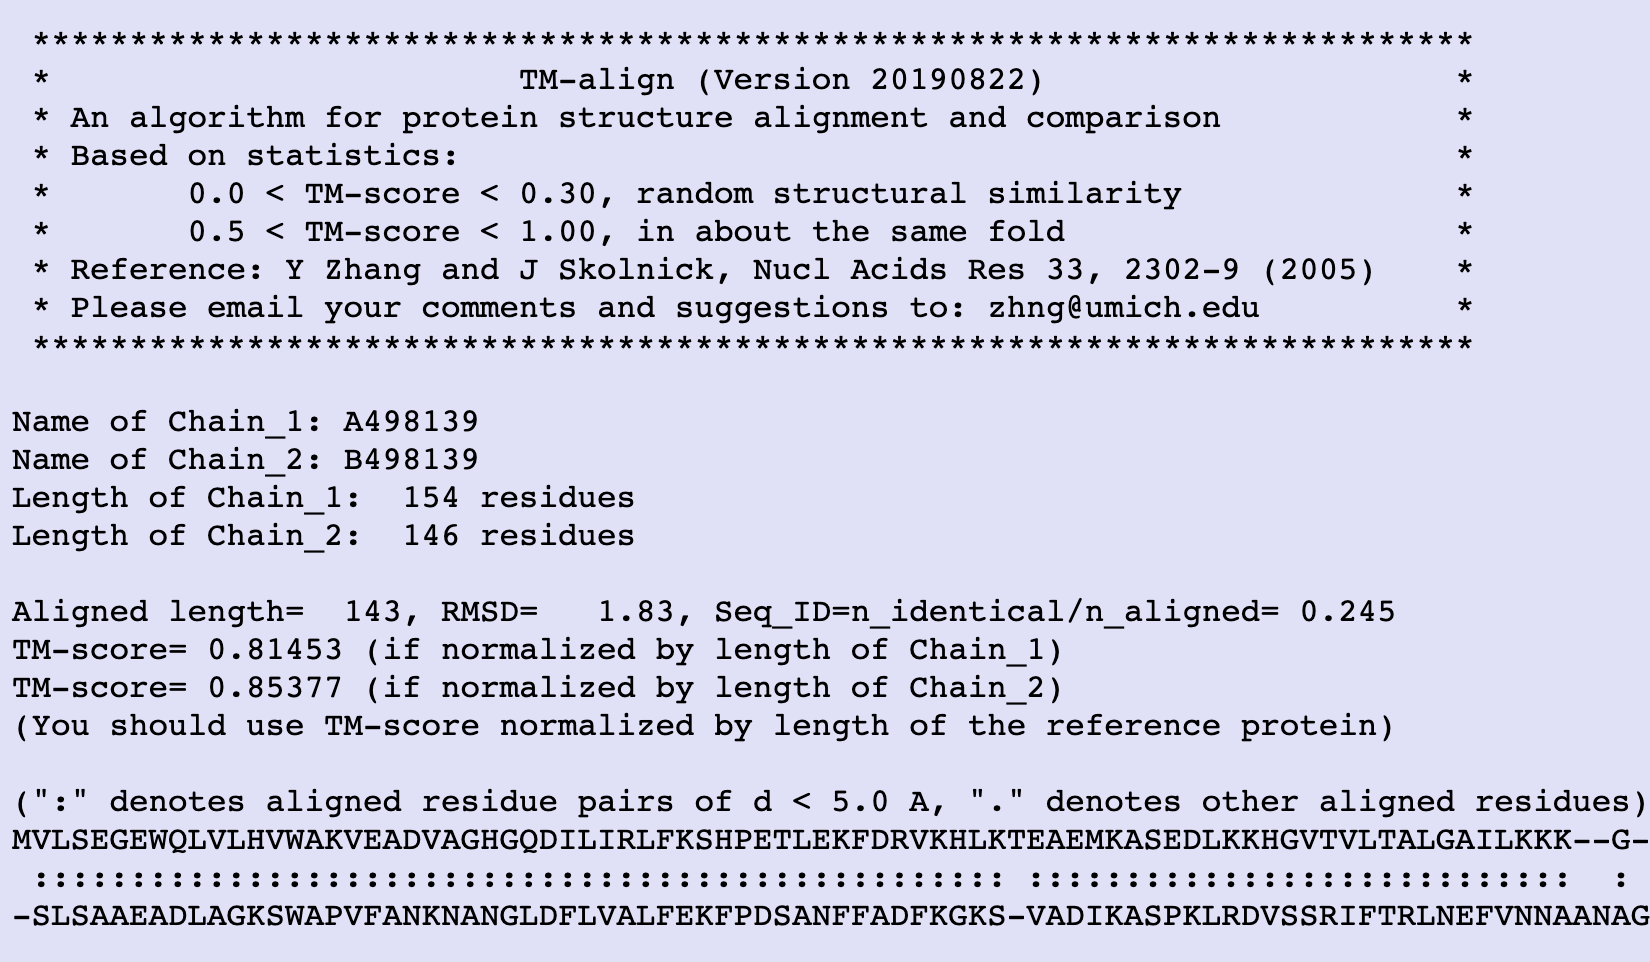
\includegraphics[width=0.8\textwidth]{TmalignResult.png}
    \caption{\label{fig:TmalignResult}Showing text result when running tmalign on the https://zhanggroup.org/TM-align/ site~\cite{zhang_tm-align_nodate}.}
\end{figure}

\clearpage

\begin{figure}[ht]
    \centering
    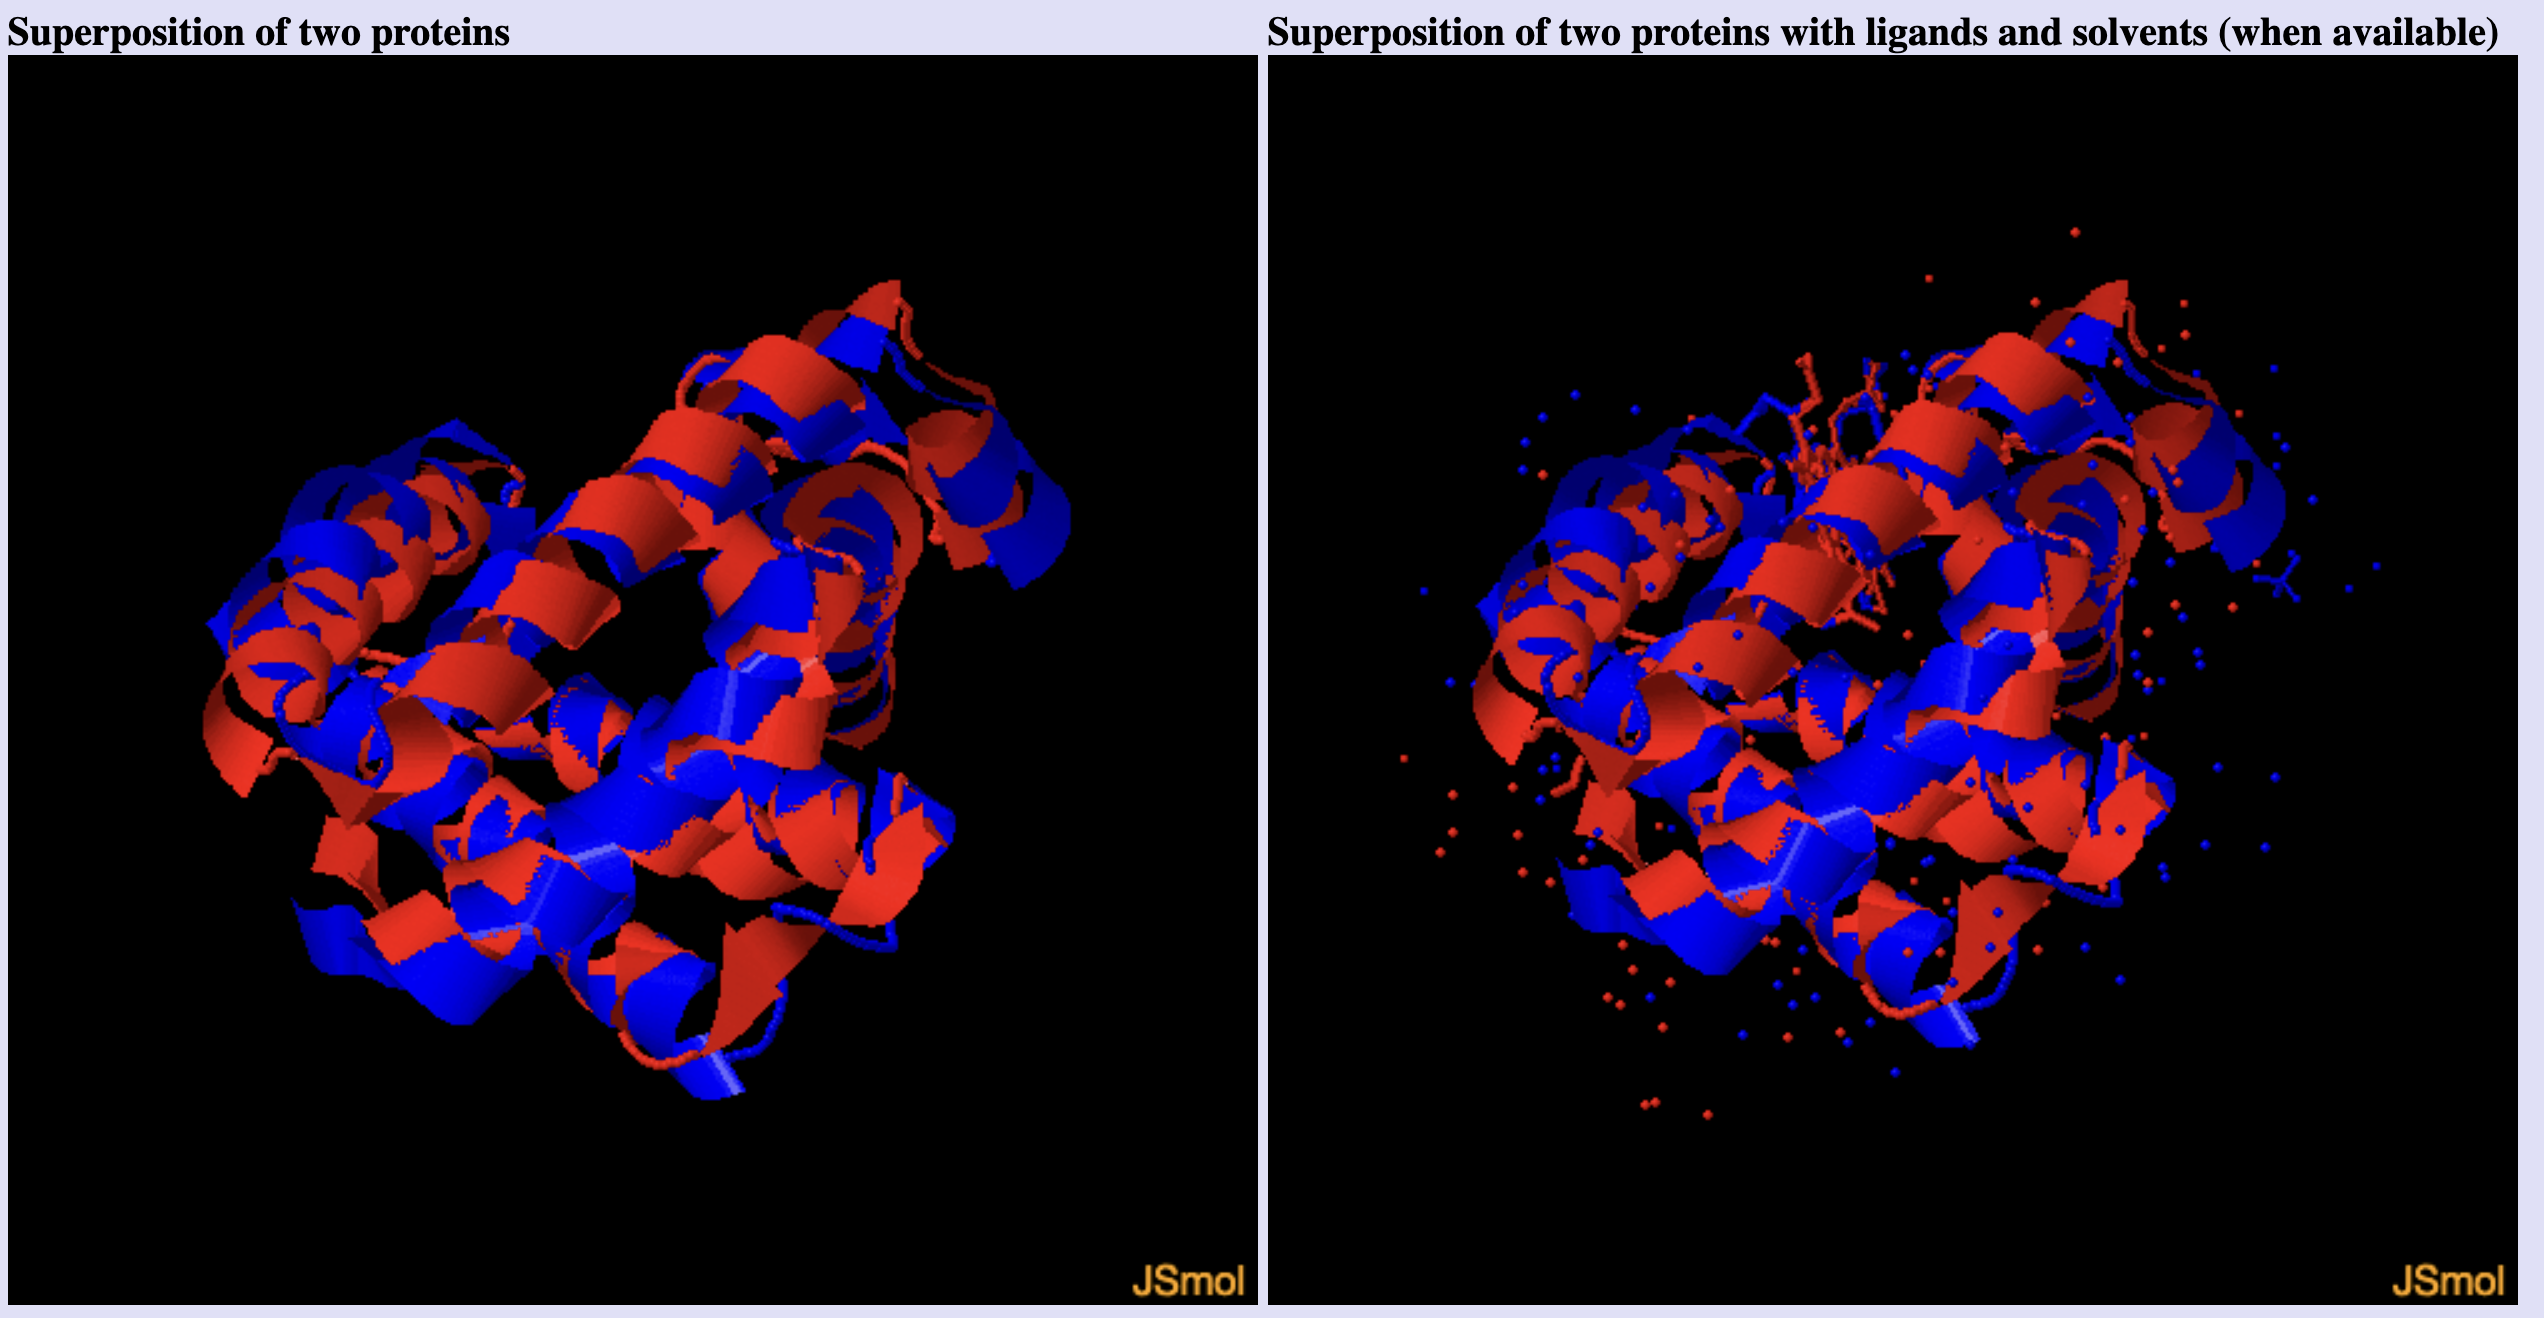
\includegraphics[width=0.8\textwidth]{TmalignVisual.png}
    \caption{\label{fig:TmalignVisual}Showing visual result when running tmalign on the https://zhanggroup.org/TM-align/ site~\cite{zhang_tm-align_nodate}.}
\end{figure}

TMalign has useful documentation on setup and example executions which helped implement it into a python program.

\subsubsection{TMalign Pythin Implementation}

First, I needed to download and set up tmalign on my computer. You can download the latest version of TM-align from the official website: http://zhanglab.ccmb.med.umich.edu/TM- align/

We then need to compile the program by running the command ”make” within the directory of tmalign. This should generate an executable file called TMalign. Now that tmalign is installed we can call the bash commands listed in the document:

\begin{lstlisting}
    TMalign chain_1.pdb chain_2.pdb
\end{lstlisting}

This will me our map step within the python function. For example the line

\begin{lstlisting}
    rdd.map(lambda tuple: TMalign(tuple[0], tuple[1])).collect()
\end{lstlisting}

which will pass in the values of the protien strucutre into the tmalign function. This functions objective is to get two files and run the bash command shown above on it:

\begin{lstlisting}
    def TMalign(tuple1, tuple2):
    with tempfile.NamedTemporaryFile() as tmp1, \
         tempfile.NamedTemporaryFile() as tmp2:
        tmp1.write(tuple1[1])
        tmp2.write(tuple2[1])
        os.system('./TMalign {} {}'.format(tmp1.name, tmp2.name))
\end{lstlisting}

\clearpage

\subsubsection{Hoppscore}

Hoppscore is a user executable written for the purpose to provide a score when passed in a pdb file which indicates the quality of a given protein. The higher the Hoppscore value, it is better for the experimental data. However, I came across some issues with setting the script up.

Here is an example of what an example hoppscore execution would look like:

\begin{lstlisting}
    hoppscore  -r 1.7 -g 12 sample.pdb 

    Output is sent to STDOUT

    hoppscore -r 1.7 -g 12 sample.pdb > sample.pdb.out
\end{lstlisting}

Program output is sent to STDOUT and looks like this:

\begin{lstlisting}
    !F - Favored, A - Allowed, U - Unfavored, D - Disallowed
    !F > 612.7, 183.3 < A > 612.7, 0 < U > 183.3, D=0
    !Avg: 183.290662650602, Sigma: 858.791452289234
    !Input File: test.pdb
    !Reference Database Resolution Limit: 17
    !phi-psi pairs: 1
    !  SS    AA   FILENAME  RES      F/Avg  Favored?
    !-----------------------------------------------
        C     D   test.pdb    2      10.19  F   2
        S     A   test.pdb    3      34.83  F   2
        G     P   test.pdb    4      99.17  F   2
        G     F   test.pdb    5       5.93  F   2
        G     E   test.pdb    6       1.01  A   1
     .
     .
     .

    !-----------------------------------------------
                                       Sum: 111
                                     Score: 1.23
\end{lstlisting}

However when attempting to install the program i failed to do so. The readme files show how to install the tool in different operating systems however i failed to do so when following the steps and there is no external help or documentation online for this tool. This can be because the program was last updated in 10/04/2013 showing that it has not been an active analysis tool recently and is not widely used.
\clearpage


\subsection{Objective Implementation}

Out of all the objectives listed in section 2.2, I will go through each one and show my implementation, thoughts, issues and any technical decisions I had to make whilst trying to achieve the objective.

\subsubsection{MapReduce Framework for Protein Analysis}

\begin{displayquote}
    Develop a software framework that suppots the Mapreduce formalism and can process
    large numbers of protein structures.
\end{displayquote}

To implement this we need to break down the objective into two parts the first part is to build a framework that supports a mapreduce formalism and the second part is to ensure that the build can process large number of protien structures. 

\subsubsection{1. Framework that Supports a MapReduce Formalism}

The first decision I have to make is to decide what software to use which can enable me to use a MapReduce formalism I concluded with two options, Hadoop and apache spark. Please refer to my Literature review on Hadoop spark and pyspark in summary spark is newer and performs quicker whilst having an API for python. Which ultimately led me to choose spark over Hadoop.

\clearpage

\subsubsection{Implementing PySpark}

\textbf{Install Java:} PySpark requires Java to run. You can download and install Java from the official website (https://www.oracle.com/java/technologies/javase-downloads.html).

\textbf{Install Apache Spark:} PySpark is built on top of Apache Spark. You can download Apache Spark from the official website (https://spark.apache.org/downloads.html). Note pick a version that matches your java version.

\textbf{Install Python:} PySpark requires Python 3.x to run. Download and install Python from the official website (https://www.python.org/downloads/).

Set environment variables: To use PySpark, you need to set environment variables for Java and Spark. On MAC OS and linux open the terminal and run the following commands:

\begin{lstlisting}[language=bash]
    export JAVA_HOME=/Library/Java/
    JavaVirtualMachines/JDKversion/Contents/Home
    export PATH=$JAVA_HOME/bin:$PATH
    export SPARK_HOME=<path_to_spark_folder>
    export PATH=$SPARK_HOME/bin:$PATH
\end{lstlisting}

On windows open command prompt and run the following commands:
\begin{lstlisting}[language=bash]
    setx JAVA_HOME "C:\Program Files\Java\jdk-16.0.2"
    setx PATH "%PATH%;%JAVA_HOME%\bin"
    setx SPARK_HOME "C:\spark-3.2.0-bin-hadoop3.2"
    setx PATH "%PATH%;%SPARK_HOME%\bin"
\end{lstlisting}

\textbf{Install PySpark:} You can install PySpark using pip using the following command:

\begin{lstlisting}[language=bash]
    pip install pyspark
\end{lstlisting}

Finally \textbf{Test PySpark:} You can test PySpark to check if all is set up correctly by opening the Python shell and running the following commands:

\begin{lstlisting}[language=bash]
    from pyspark.sql import SparkSession
    spark = SparkSession.builder.appName("test").getOrCreate()
    df = spark.range(10)
    df.show()
\end{lstlisting}

The above code creates a SparkSession which is a distributed computing framework that supports a MapReduce formalism.

The code creates a SparkSession with the name "test". Providing a way to interact with Spark's features. Once the SparkSession is created, the code generates a DataFrame Which yields ten rows with values from 0 to 9. Finally, the code prints the contents using the show() method. Overall this is a stepping stone to a Framework that supports MapReduce formalism.

\clearpage

\subsubsection{2. Process Large Numbers of Protein Structures}

The second part of the objective is to ensure that we can process large numbers of protein structures. To do this we need to optimize our Spark job and cluster configuration. Some actions fall outside of our ability to execute, while others can be considered during the planning phase before coding, and some can be implemented directly into the code itself.

\subsubsection{Can not implement}
\textbf{Cluster Configuration:} I initially aimed to use a YARN implementation that allows you to dynamically share and centrally configure the same pool of cluster resources between all frameworks that run on YARN.~\cite{goyal_spark_2018} These are the issues I ran across:

\begin{enumerate}
    \item \textbf{Configuration:} Yarn requires additional configuration beyond what is required for a standalone Spark cluster. You need to configure Yarn-specific settings such as memory allocation and container sizes, as well as Spark-specific settings such as executor and driver memory.
    \item \textbf{Resource Management:} Yarn is responsible for managing resources for multiple applications running on a shared cluster. This can make it more difficult to manage resource allocation and ensure that each application has access to the resources it needs.
    \item \textbf{Monitoring:} Because Yarn is managing resources for multiple applications, it can be more difficult to monitor the performance of individual applications. You need to look at both Yarn-level metrics and Spark-level metrics to get a complete picture of performance.
    \item \textbf{Troubleshooting:} When issues arise in a Yarn-managed cluster, it can be more difficult to troubleshoot the problem. You need to determine whether the issue is related to Yarn or Spark, and then diagnose the problem accordingly.
\end{enumerate}

Due to a smaller-scale workload and a simpler, more flexible, and more cost-effective option, a standalone Spark cluster is be a better fit.

\textbf{Data Serialisation:} Serialisation is the process of converting data structures into a format that can be easily transmitted over the network. By default, PySpark uses Python's pickle library for serialisation, which can be slow for large datasets. You can improve serialisation performance by using more efficient serialisation formats like Avro or Parquet. However, I came across some issues:

Due to the amount and complexity of the protein structure analysis data, serialisation and deserialization can result in performance overhead. Even though both are often used, they might not have the same level of tooling and support as other formats, like CSV, JSON, or text. Working with data in these formats could become more challenging as a result. Ultimately, both can make your data processing pipeline more complex. To use these formats, for instance, you might need to create your own serialisation and deserialization algorithms or set up your data processing systems.

Thus, I have decided to use Python's pickle library for serialization.

\clearpage

\subsubsection{Before Implementing the Code}
\textbf{Hardware Configuration:} Make sure your cluster has enough CPU, RAM, and disc resources to manage the demand. SSDs can also be used to do faster I/O operations and faster disc access. So, we must make sure that the hardware running the framework satisfies the requirements.

We must first examine the prerequisites for running PySpark to accomplish this:

\begin{itemize}
    \item A 64-bit operating system e.g., macOS, Linux, or Windows
    \item At least 8 GB of RAM
    \item A multi-core processor e.g., Intel Core i5 or i7
\end{itemize}

\subsubsection{Whilst Implementing Code}
These are some features of pyspark that we can implement into our code to ensure that optimize our Spark job and cluster configuration.

\textbf{Caching:} Caching is an optimization technique that involves storing intermediate results in memory to avoid recomputation. Caching is particularly useful when you have iterative algorithms that reuse the same data multiple times. You can use the cache function in PySpark to cache Resilient Distributed Datasets or DataFrames.

\textbf{Partitioning:} Partitioning the input data can significantly improve performance, especially for large datasets. Partitioning involves splitting the data into smaller chunks and processing them in parallel.

\clearpage

\begin{table}[ht!]
    \begin{center}
        \label{tab:partitioning}
        \begin{tabular}{p{0.6\linewidth}|p{0.35\linewidth}}
            Partitioning Function & Description\\
            \hline
            \\
            hash() & Hashes the keys and partitions the data based on the hash value of the key. It is the default partitioning function in PySpark.
            \\
            \hline
            \\
            range() & Partition the data based on the range of the key values. For example, if the key values range from 1 to 100, and there are 4 partitions, the first partition will contain keys from 1 to 25, and so on.
            \\
            \hline
            \\
            round robin() & This function partitions the data in a round-robin fashion. For example, if there are 3 partitions, the first partition will contain the first record, the fourth record, the seventh record, and so on.
            \\
            \hline
            \\
            custom() & This function allows you to define your own partitioning logic by implementing the getPartition(key) method.
        \end{tabular}
        \caption{\label{partitioning}Showing examples of pyspark partitioning functions and what they do.}
    \end{center}
\end{table}

\subsubsection{Amended Code to Handle Large Amounts of Protein Data}

\begin{lstlisting}
    proteinfiles = spark.read.format("text").load(path)
    processedproteins = protein_files.rdd.map(processprotein)
\end{lstlisting}

These are two lines of code that will allow the ability to handle large amounts of protein data. 

Where proteinfiles holds the information of the protein structure. We then would pass this into a map function that will conduct processes on the protein structure data. Finally performing a .collect() function will save the results of the processed data into processed proteins.

Ultimately using this with conjunction of the code used to test pyspark we end up with a framework that supports the Mapreduce formalism and can process large number of protein structures.

\clearpage

\subsubsection{Parallelized Protein Analysis with MapReduce}

\begin{displayquote}
    Implement a distributed computing system using MapReduce to parallelize protein structure analysis across multiple computing nodes.
\end{displayquote}

To implement a distributed computing system using MapReduce to parallelize protein structure analysis across multiple computing nodes using PySpark, we need complete the following steps:

\begin{enumerate}
    \item Setup a PySpark cluster with multiple worker nodes.
    \item Write a Map function to parse the protein structure data and extract the relevant features.
    \item Write a Reduce function to combine the results from the Map function.
    \item Load the protein structure data into PySpark RDDs.
    \item Create a function that can process protein structures.
    \item Apply the Map function to each protein structure RDD in parallel.
    \item Apply the Reduce function to combine the results from the Map function.
    \item Save the output to a distributed file system.
\end{enumerate}

The following code has been taken from my lines program which is intended to print the number of lines each pdb file contains which completes the steps provided above

\begin{lstlisting}
    from pyspark.sql import SparkSession
    from pyspark.sql.types import StringType
    import os
    from pathlib import Path
    import tempfile

    def main(spark):
        directory = ("/PROJECT/Programs/Lines/PDBsDirectory/*")
        tempdirectory = "/PROJECT/Programs/Lines/PDBsfromRDD"

        rddkeyvalue = spark.sparkContext.wholeTextFiles(directory)

        def numberoflines(filename, filecontent):
            with tempfile.NamedTemporaryFile() as tmp:
                tmp.write(filecontent)
                os.system("wc -l "+ tmp.name)

        r = rddkeyvalue.map(lambda x: numberoflines(x[0], x[1]))
        r = r.collect()
    if __name__ == '__main__':
        spark = SparkSession.builder.appName('PDB').getOrCreate()
        main(spark)

\end{lstlisting}

\clearpage

\subsubsection{PySpark Cluster Setup}

The SparkSession object is a higher-level interface to create a Spark application with SparkContext, which provides a unified entry point to interact with the Spark cluster.

We use the builder API to create a SparkSession instance and set the application name to "PDB". The getOrCreate method creates a new SparkSession instance or reuses an existing one if one already exists. This creates a SparkSession with all the necessary configurations and settings for connecting to the Spark cluster.

When we execute the code, the SparkSession instance is created and the worker nodes are launched, enabling distributed computing across the cluster.

\subsubsection{Map Function}
The numberoflines function takes a folder's path and the values within the protein structure and creates a temp file in which it writes the contents of the protein structure. The temp file is then used to get the number of lines with the shell command "wc -l 'tempfilename'".

Once the numberoflines function has been defined, we can apply it to each protein structure file in parallel using the Map function in Spark.


\subsubsection{Reduce Function}
The code provided does not include an explicit implementation of a Reduce function. However, you can write a Reduce function using PySpark's reduce function, which would result in the same response if needed to return the number of lines.


\subsubsection{PySpark RDDs}
The code provided, loads protein structure data by using the wholeTextFiles function to read all the files in a directory as an RDD of key-value pairs, where the key is the filename and the value is the contents of the file.

\subsubsection{Save to Distributed File System}
The code provided does not include any code to save the output to a distributed file system. However, you can use PySpark's saveAsTextFile function to save the output as text files in a distributed file system.
\clearpage

\subsubsection{Optimization for Faster Protein Analysis}

\begin{displayquote}
    Optimize the software framework to reduce the processing time required for protein structure analysis.
\end{displayquote}

I will now present the first version of my lines programs and explain the features I changed so that the framework will be more optimized to reduce the processing time required for protein structure analysis.

\begin{lstlisting}
    from pyspark.sql import SparkSession
    from pyspark.sql.types import StringType
    import os
    import shutil
    from pathlib import Path


    def main(spark):
        directory = ("/Programs/Lines/PDBsDirectory")
        tempdirectory = "/PROJECT/Programs/Lines/PDBsfromRDD"

        for file in os.listdir(os.fsencode(directory)):
            filename = os.fsdecode(file)
            if filename.endswith(".DS_Store"):
                continue
            rdd = spark.read.text("/PDBsDirectory/"+filename)
            rdd = rdd.map(lambda x: x[0])
            if os.path.exists(tempdirectory):
                shutil.rmtree(tempdirectory)
            rdd.saveAsTextFile(tempdirectory)
            os.system("wc -l "+tempdirectory+"/part-00000")


    if __name__ == '__main__':
        # This creates a local cluster
        spark = SparkSession.builder.appName('PDB').getOrCreate()
        main(spark)
\end{lstlisting}

\clearpage

\subsubsection{Issues with code}
We have instantiated a for loop which loops through all the files in the PDBsDirectory the code then reads each file in the PDBsDirectory directory and loads it into an RDD using spark.read.text ignoring any files that end with DSStore which is one of the outputs returned from saveAsTextFile. This operation can be time-consuming for large files because it involves reading the entire file into memory as a single string. This is not efficient for processing large files.

The code then saves the RDD to the PDBsfromRDD directory using rdd.saveAsTextFile but we need to check if this directory exists already, deleting it if so, as for the next pdb file in the PDBsDirectory, we will need to cast saveAsTextFile to this which requires that folder to not exist in the first place. SaveAsTextFile function can be expensive because it involves writing the entire RDD to disk.

Finally, if there are a lot of files in PDBsDirectory the for loop will need to go through each one whilst also running shutil.rmtree which is not efficient as some operations are being run each iteration which we can remove.

\clearpage

\subsubsection{Improvement Using wholeTextFiles()}

wholeTextFiles() can be used instead of textFile() to read all files within a directory as a single RDD. wholeTextFiles() reads the files in the specified directory and returns an RDD where each element is a tuple of (filename, contents), where filename is the name of the file and contents is the entire contents of the file as a single string.

This eliminates the need to have a for loop to go through the directory as we can read each file in the directory using wholeTextFiles() and a wildcard '*' in the directory path for example directory = "/path/*" which will select all the files in that path.

As we have the name and content of the file we can remove saveAsTextFile() as we can pass the file name into the map function thus casting the shell command on the file.

This will result in the following code:

\begin{lstlisting}
    from pyspark.sql import SparkSession
    from pyspark.sql.types import StringType
    import os
    import shutil
    from pathlib import Path


    def main(spark):
        start = time.time()
        directory = ("/PROJECT/Programs/Lines/PDBsDirectory/*")

        rddkeyvalue = spark.sparkContext.wholeTextFiles(directory)

        def numberoflines(k):
            os.system("wc -l "+ k[40:])
        
        rddkeyvalue.map(lambda x: numberoflines(x[0])).collect()


    if __name__ == '__main__':
        # This creates a local cluster
        spark = SparkSession.builder.appName('PDB').getOrCreate()
        main(spark)
\end{lstlisting}

\clearpage

\subsubsection{Integrate API for PDB access}
\begin{displayquote}
    Integrate a PDB file download and search from the RCSB API for efficient data access.
\end{displayquote}

As the software framework is dependent on what files are currently loaded into the correct folders this objective is important as it is an easy way for the researcher to download pdb files without having to access the website.

The objective is to work with the RCSB protein data bank website using their provided API. Please refer to my Literature review of the website for a better understanding of what it holds and the features it provides. In summery, the RCSB Protein Data Bank website is a comprehensive resource that provides access to 3D structural data of proteins, nucleic acids, and complex assemblies. It is a valuable tool for researchers in the fields of biochemistry, biophysics, and molecular biology.

The RCSB site provides many APIs including:
\begin{itemize}
    \item Data API
    \item Search API
    \item ModelServer API
    \item VolumeServer API
    \item 1D Coordinate Server
\end{itemize}

The features that are required for this objective and are also the main features that power rcsb.org are, File Download Services which, serves to download the pdb file of a provided protein structure. Search API serves to find out what identifiers match a certain search condition.

\clearpage

\subsubsection{File Download Services}

The file download service provides the ability to download a file that the website contains given the correct parameters. This is important as it will allow the researchers to use the API to download any required files without needing to access the website. 

The following URL is an example of how to download a .pdb file in this case 4hhb.pdb:

\begin{lstlisting}
    https://files.rcsb.org/download/4hhb.pdb
\end{lstlisting}

There are a few different options when downloading files from the website:

\begin{table}[h]
    \begin{center}
        \begin{tabular}{ |p{5.5cm}|p{2.5cm}|p{6cm}|  }
            \hline
            \multicolumn{3}{|c|}{PDB entry files} \\
            \hline
            File Format&Compression&Example URL\\
            \hline
            Biological Assembly File in PDB&Uncompressed&/download/1hh3.pdb1\\
            \hline
            Biological Assembly File in PDB&Compressed&/download/1hh3.pdb1.gz\\
            \hline
            Biological Assembly File in PDBx/mmCIF&Uncompressed&/download/5a9z-assembly1.cif\\
            \hline
            Biological Assembly File in PDBx/mmCIF&Compressed&/download/5a9z-assembly1.cif.gz\\
            \hline
            PDB&Compressed&/download/4hhb.pdb.gz\\
            \hline
            PDB&Uncompressed&/download/4hhb.pdb\\
            \hline
            PDBx/mmCIF&Compressed&/download/4hhb.cif.gz\\
            \hline
            PDBx/mmCIF&Uncompressed&/download/4hhb.cif\\
            \hline
            XML&Compressed&/download/4hhb.xml.gz\\
            \hline
            XML&Compressed&/download/4hhb.xml\\
            \hline
        \end{tabular}
        \caption{\label{DownloadPDB}Showing different type of downloads options using the Download Serivce~\cite{bank_file_nodate}.} 
    \end{center}
\end{table}
    
Depending on what is put after the download in the URL we will get a different download. The table highlights some of the main File formats and examples of how to use the URL to download them.

\clearpage

\subsubsection{Implementing Download Service into Python}

Using this we can retrieve the data for a given pdb file name and write it into a file and save it to the path given:

\begin{lstlisting}
    import requests

    apicall = 'https://files.rcsb.org/download
    /{}.pdb'.format(pdbfile)

    response = requests.get(apicall)

    with open('path' + pdbfile + '.pdb', 'wb') as f:
        f.write(response.content)

\end{lstlisting}

The RCSB site holds an extremely vast amount of pdb files we can see all current PDB ids by going to:

\begin{lstlisting}
    https://data.rcsb.org/rest/v1/holdings/current/entry_ids
\end{lstlisting}

This brings in the need for the search API. As it is not good to assume that the user will have the name for each file they would like to download.

\clearpage

\subsubsection{Search API}

The Search API accepts HTTP GET or POST requests with JSON payloads. In GET method, search request should be sent as a URL-encoded query string in json parameter~\cite{burley_rcsb_2019}\cite{rose_rcsb_2021}: 

\begin{lstlisting}
    https://search.rcsb.org/rcsbsearch/v2/query?json={search-request}
\end{lstlisting}

A search request is a complete specification of what should be returned in a result set. The search request is represented as a JSON object. The building blocks of the request are~\cite{burley_rcsb_2019}\cite{rose_rcsb_2021}:

\vspace{40px}

\begin{table}[ht!]
    \begin{center}
        \label{tab:json}
        \begin{tabular}{p{0.6\linewidth}|p{0.35\linewidth}}
            Context & Description\\
            \hline
            \\
            return type (Required) & Specifies the type of the returned identifiers, e.g. entry, polymer entity, assembly, etc.
            \\
            \hline
            \\
            query (Optional) & Specifies the search expression. Can be omitted if, instead of IDs retrieval, facets or count operation should be performed. In this case the request must be configured via the request options context.
            \\
            \hline
            \\
            request options (Optional) & Controls various aspects of the search request including pagination, sorting, scoring and faceting. If omitted, the default parameters for sorting, scoring and pagination will be applied.
            \\
            \hline
            \\
            request info (Optional) & Specifies an additional information about the query, e.g. query id. It's an optional property and used internally at RCSB PDB for logging purposes. When query id is sent with the search request, it will be included into the corresponding response object.
        \end{tabular}
        \caption{\label{json}Aspects that a valid json for the search api on RCSB can hold~\cite{burley_rcsb_2019}\cite{rose_rcsb_2021}.}
    \end{center}
\end{table}

\clearpage

Here is an example valid JSON and the response for the results shown when searching for thymidine kinase~\cite{burley_rcsb_2019}\cite{rose_rcsb_2021}:

\begin{lstlisting}
  "query": {
    "type": "terminal",
    "service": "full_text",
    "parameters": {
      "value": "thymidine kinase"
    }
  },
  "return_type": "entry"
\end{lstlisting}

\vspace{40px}

This is the response receive back:

\begin{lstlisting}
  "query_id" : "f3424f3f-a69a-4b70-96ee-df9fb8db7558",
  "result_type" : "entry",
  "total_count" : 57547,
  "result_set" : [ {
    "identifier" : "2UZ3",
    "score" : 1.0
  }, {
    "identifier" : "2B8T",
    "score" : 0.9175522850503486
  }, {
    "identifier" : "2WVJ",
    "score" : 0.898559256390395
  }, {
    "identifier" : "2J87",
    "score" : 0.602571649883811
  }, {
    "identifier" : "2VTK",
    "score" : 0.3646165762974438
  }, {
    "identifier" : "1XBT",
    "score" : 0.2990240123934934
  }, {
    "identifier" : "1KIM",
    "score" : 0.24848954298993028
  }, {
    "identifier" : "1E2J",
    "score" : 0.18949651432997677
  }, {
    "identifier" : "1P6X",
    "score" : 0.08545313710302091
  }, {
    "identifier" : "2QQE",
    "score" : 0.0
  } ]
\end{lstlisting}

We get the pdb identifier and the score of how relatable it is to the search value. This is helpful as now we can in theory download each result as we have the identifier associated with them. For example: https://files.rcsb.org/download/2UZ3.pdb

\subsubsection{Implementing Search API in Python}

Before starting the python program we need to create a valid JSON file. Using the examples provided by the RCSB API documentation found here https://search.rcsb.org/basic-queries We can set up a JSON file that looks like the following:

\begin{lstlisting}
   "query":{
      "type":"terminal",
      "service":"full_text",
      "parameters":{
         "value":"vinay"
      }
   },
   "return_type":"entry"
\end{lstlisting}

We now need to create a following python program that can use the following JSON file and execute a get request to the API. The following program was created: 

\begin{lstlisting}
    def main(folder, value):
    
        jsonfile = 'Search.json'
        directory = (path)
    
    
        with open(file=jsonfile, mode="r") as jsonFile:
            data = json.load(jsonFile)
    
        data['query']['parameters']['value'] = value
    
    
        with open(file=jsonfile, mode="w") as jsonFile:
            json.dump(data, jsonFile)
    
        #fix to make the values in data 
        #not use ' qoutes but use "" qoutes instead
        data = json.dumps(data)
    
        newdata = urllib.parse.quote(data)
        apicall = 
        'https://search.rcsb.org/rcsbsearch/v2
        /query?json={}'.format(newdata)
    
    
        result = requests.get(apicall)
        result = result.json()
        for x in result["result_set"]:
            print(x)
    if __name__ == '__main__':
        globals()[sys.argv[1]](sys.argv[2], sys.argv[3])
    #Example run line: 
    # python3 searchpdbfiles.py main PDBsDirectory2 vinay
    
\end{lstlisting}

In this program, we first define the URL of the RCSB PDB API endpoint. We then open and change the value of the search filter to what is provided and load the JSON file from a query dictionary to a JSON string using json.dumps(). The urllib.parse.quote() method is used to URL-encode the search query JSON string. The script sends a GET request to the API using the requests.get() method with the apicall URL. Finally retrieving the results and printing them.

\subsubsection{Issues with Creating a Valid JSON}

I came across an issue when creating a valid JSON to pass into the Search API. Currently, the JSON file is only allowing the search for one value. However, there is a vast number of other filters and search options a researcher can use when browsing the pdb bank. Therefore I decided to consolidate with my supervisor to determine some useful filter options for the researchers to use whilst working with the framework. Two useful filters included:

\begin{itemize}
    \item R Factor
    \item Date of Deposition
\end{itemize}

This required multiple filters in one JSON query the value, R factor and Date of Deposition. This was found difficult to create a valid JSON, as the documentation uses high-level biology terms which made it hard to look for exactly what I needed. I first broke down the problem by looking at how to translate these filter terms into a valid JSON format~\cite{burley_rcsb_2019}. I found that: 

\begin{itemize}
    \item reflns.pdbx Rmerge I obs is a measure of the quality of a protein structure, specifically the average R-merge value of the observed reflections. R-merge is a statistical parameter that is used to evaluate the agreement between multiple observations of a diffraction spot. A lower value of reflns.pdbx Rmerge I obs generally indicates a better quality protein structure~\cite{worldwide_protein_data_bank_consortium_pdbxmmcif_nodate}.
    \item rcsb accession info.initial release date is the date when a protein structure was first released to the RCSB PDB. This is the date when the protein structure was deposited in the PDB for the first time, and it is assigned by the depositor. The date is in the format YYYY-MM-DD\cite{worldwide_protein_data_bank_consortium_pdbxmmcif_nodate}.
\end{itemize}

\clearpage

The documentation provides an 'Open in Editor' button which allows an easy and effective way of editing JSON and sending it through to the API for a response.

\begin{figure}[ht]
    \centering
    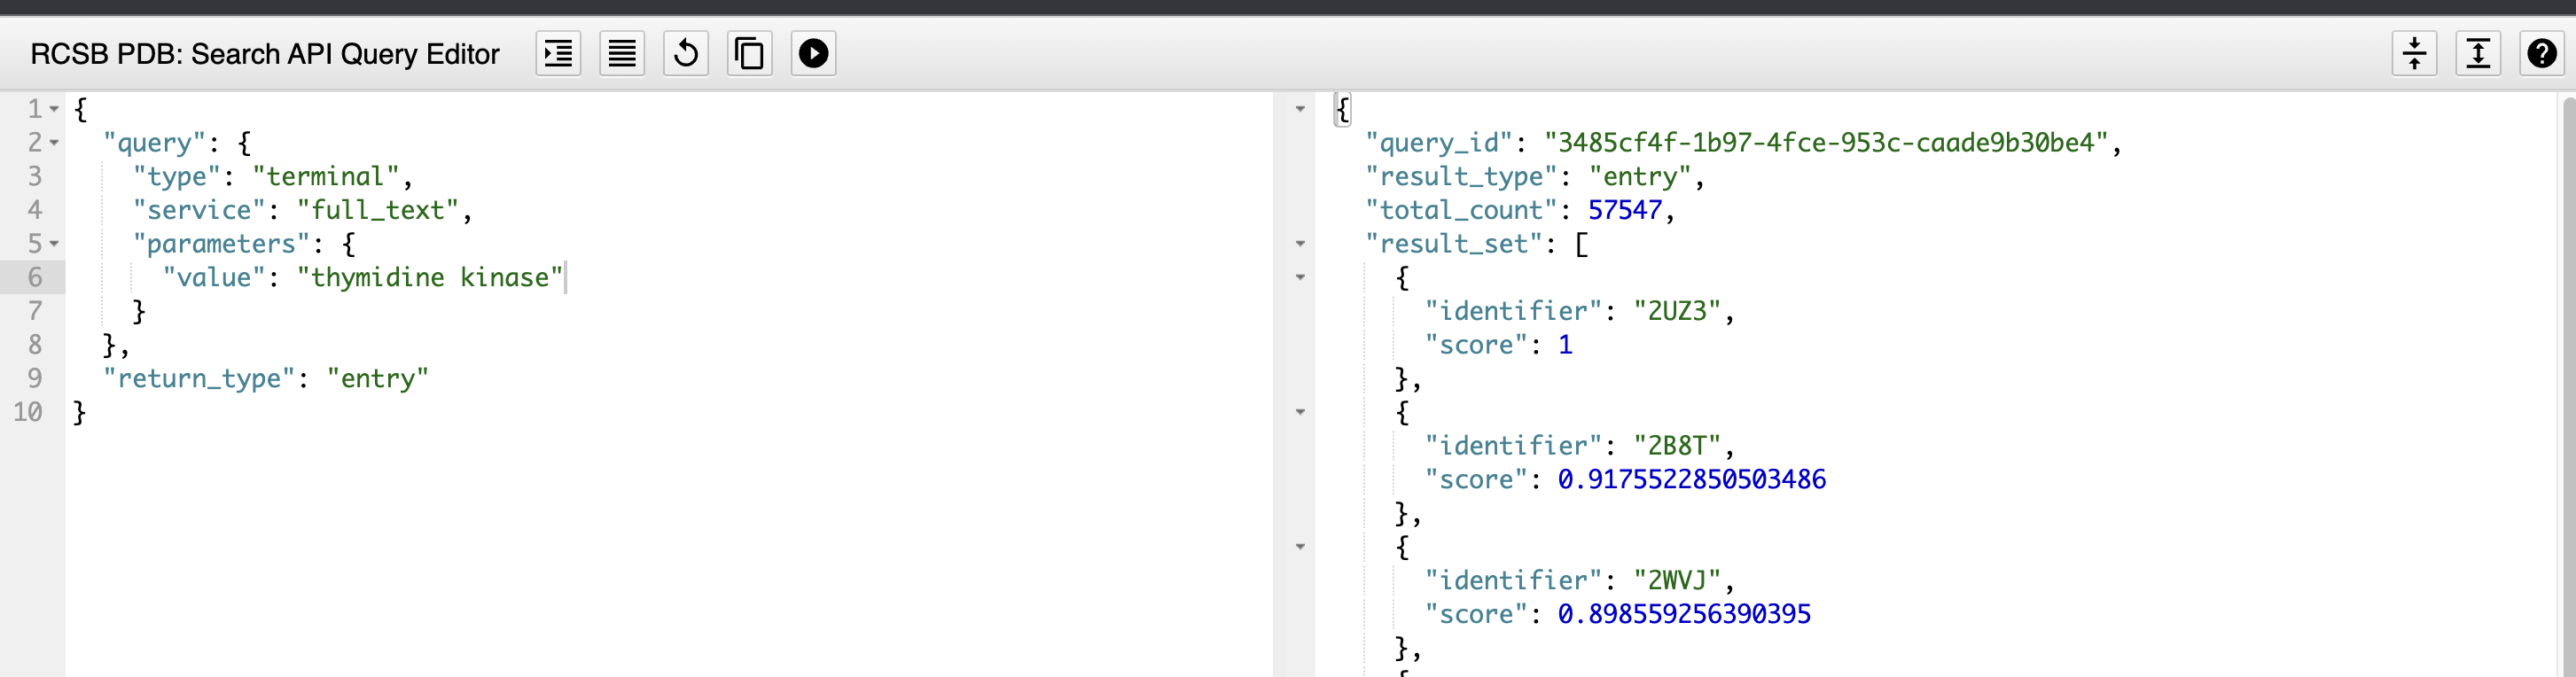
\includegraphics[width=1\textwidth]{SearchAPIEditor.png}
    \caption{\label{fig:SearchAPIEditor}Showing the User interface of the editor for the RCSB Search API~~\cite{burley_rcsb_2019}\cite{rose_rcsb_2021}.}
\end{figure}

It provides the user with error messages if the entered JSON on the left-hand side is incorrect. However, this was found to be not helpful as the messages were vague. Seeing this was not helping I decided to investigate the RCSB pdb bank website more specifically looking at the API requests being sent on the website by investigating through the advanced search using the network tab.

I first created a search using the advanced search button that fulfilled the filters I am attempting to create in JSON format.

\begin{figure}[ht]
    \centering
    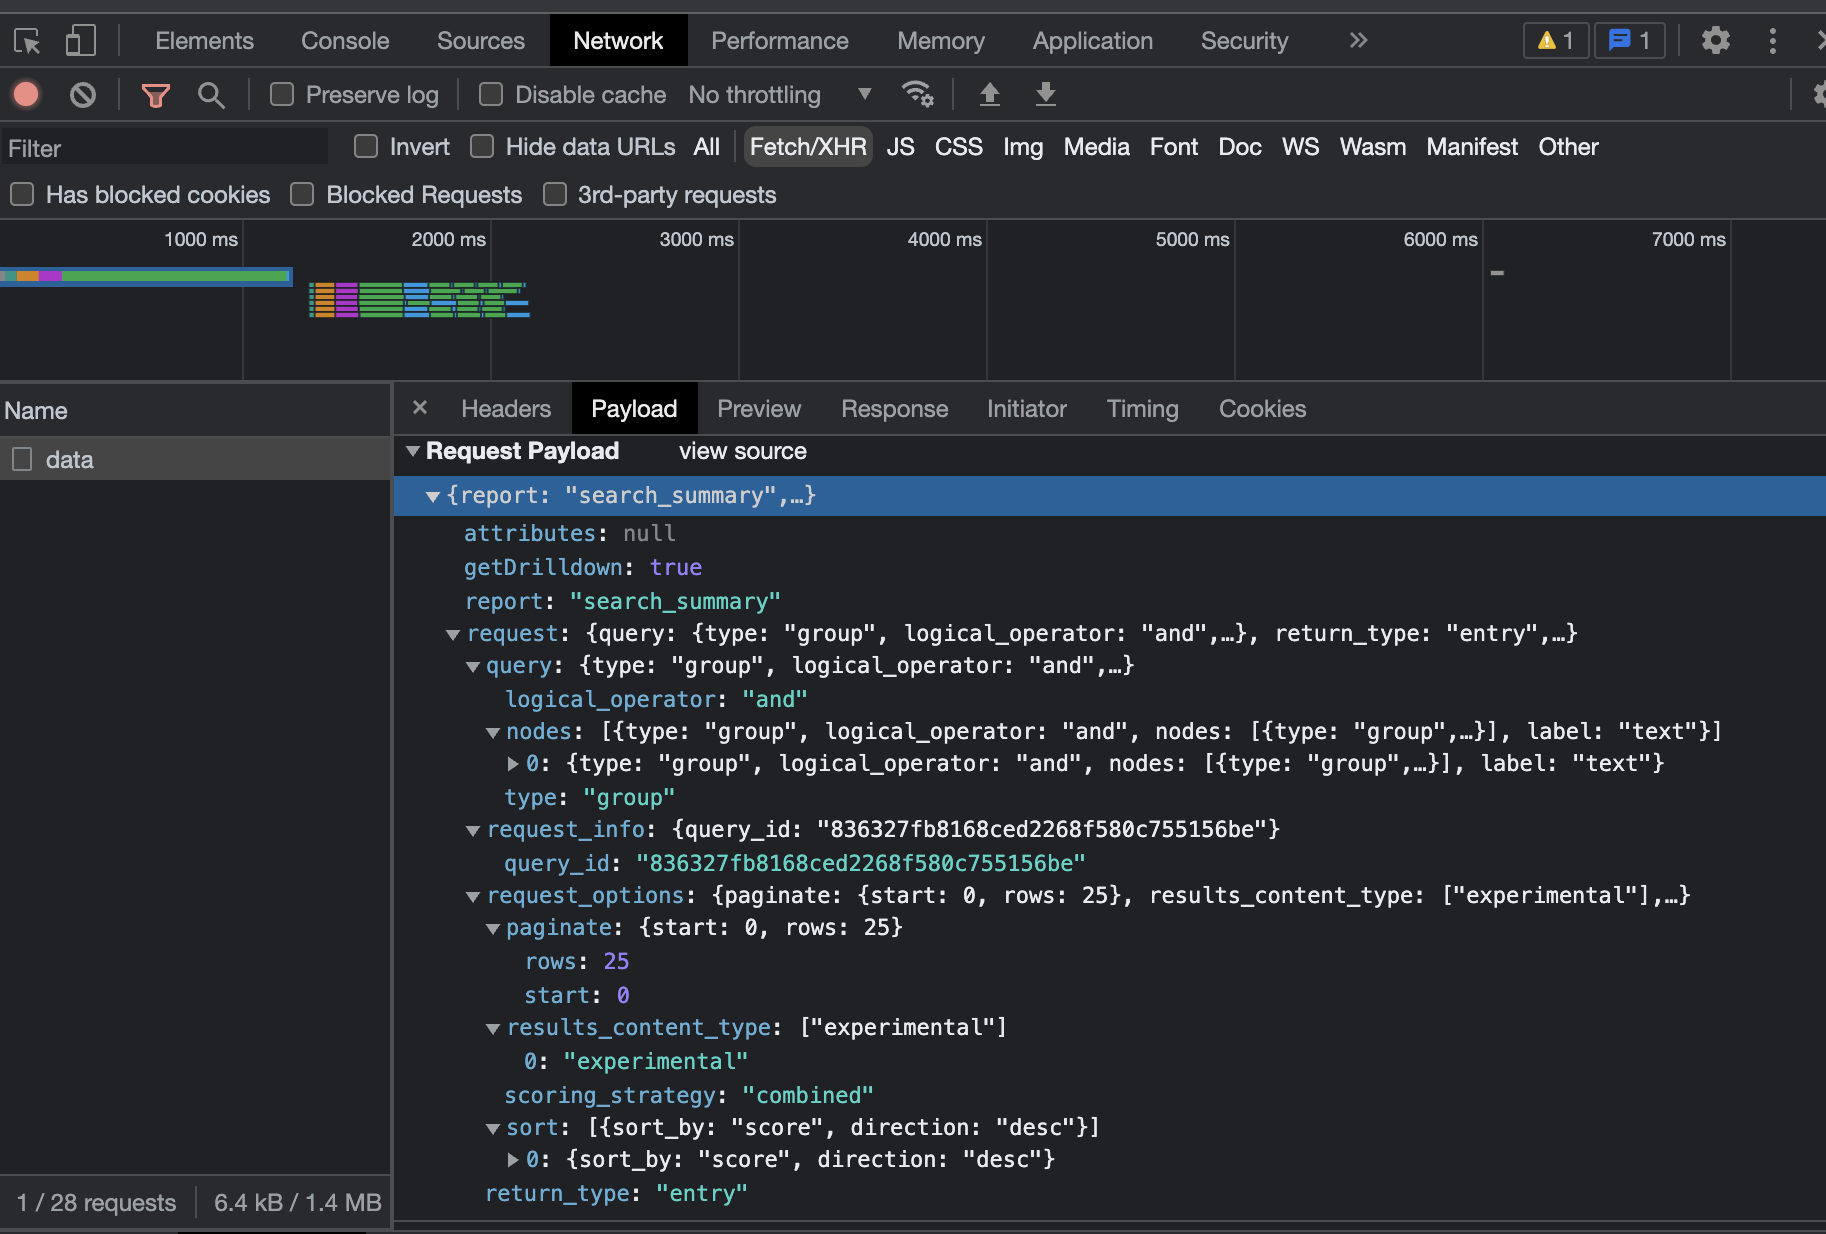
\includegraphics[width=0.5\textwidth]{payload.png}
    \caption{\label{fig:payload}Payload for when filtering through value date of deposition and rfactor}
\end{figure}

\clearpage

This payload provided me with a valid JSON with the correct filters I require however, this JSON had lots of extra components that I did not require. So using the editor, documentation and valid JSON provided by the payload I created a valid JSON that filters on the three criteria Value, Rfactor and Date of Deposition which is the following:

\vspace{30px}

\begin{lstlisting}
    "query": {
      "type": "group",
      "logical_operator": "and",
      "nodes": [
        {
          "type": "group",
          "logical_operator": "and",
          "nodes": [
            {
              "type": "terminal",
              "service":"full_text",
              "parameters": {
                "value":"covid"
              }
            },
            {
              "type": "terminal",
              "service": "text",
              "parameters": {
                "attribute":"reflns.pdbx_Rmerge_I_obs",
                "operator":"greater",
                "negation":false,
                "value":0.2
              }
            }
          ]
        },
        {
          "type": "terminal",
          "service": "text",
          "parameters": {
            "attribute": "rcsb_accession_info.initial_release_date",
            "operator": "less",
            "value": "2019-08-20"
          }
        }
      ]
    },
    "return_type": "polymer_entity"
\end{lstlisting}

\clearpage

\subsubsection{Explaining the Query}

\textbf{query}: This is the main component of the JSON, which specifies the search criteria. It consists of three parts:

\begin{enumerate}
    \item \textbf{type:} This specifies that the query is a group query, which means that it consists of multiple sub-queries that are combined using a logical operator.
    \item \textbf{logical operator:} This specifies that the logical operator used to combine the sub-queries is "and". This means that all the sub-queries must be true for a protein structure to be included in the search results.
    \item \textbf{nodes:} This is an array of sub-queries, each of which is also a group query with two sub-nodes. The first sub-node is a query to search for the term "covid" in any text field and the second sub-node is a query to filter for protein structures with a reflns.pdbx Rmerge I obs value greater than 0.2. The second group query is then combined with a third sub-node, which is a terminal query to filter for protein structures with an initial release date less than 2019-08-20.
\end{enumerate}

Finally, \textbf{return type:} This specifies the type of entity that should be returned in the search results. In this case, the return type is "polymer entity", which means that the search results will only include polymer entities, which are protein or nucleic acid molecules with a defined sequence.
\clearpage

\subsubsection{User Interface for Protein Analysis}
\begin{displayquote}
    Design an interface that allows users to manipulate the pdbs that are being passed into
    the executable for protein structure analysis.
\end{displayquote}

The framework is dependent on what files are present in the correct folder for the functions to work. This creates the need for a user interface for an easy approach to manipulating these folders to the researchers' needs. Before beginning the user interface I needed some functions that will be used when interacting with the user interface. Here is a list of all the functions I would like the user interface to inherit:

\begin{itemize}
    \item Clear all PDB files in folders
    \item Remove One or more specific pdb file in folders
    \item Return all values within the folder
    \item Add one or more specific pdb files in folders
    \item Search pdb file using API
    \item Search and download pdb file from API into the folder
\end{itemize}

After implementing these functions in python we need to create a user interface that can inherit these functions.

\subsubsection{Implementing Functions For User Interface}

There is no need to implement the Search pdb file function using API as we already have please refer to Integrate API for PDB access objective implantation.

\subsubsection{Clear all PDB files in folders}

This is the following program as the folder should only contain pdb files we don't need to specify what type of files to remove:

\begin{lstlisting}
    import os
    import sys

    def main(folder_path):
    # iterate through files and subdirectories in the provided folder
    for root, dirs, files in os.walk(folder_path):
        for file in files:
            # delete the file
            os.remove(os.path.join(root, file))

    if __name__ == '__main__':
    globals()[sys.argv[1]](sys.argv[2])

    #Example run line: python3 emptypdbfolder.py main PDBsDirectory1   

\end{lstlisting}

\subsubsection{Return all values within folder}

This is the following program as the front end has not been created yet I have left the return as print but is subject to change:

\begin{lstlisting}
    import os
    import sys

    def main(folderpath):
        for file in os.listdir(folderpath):
            print(file)

    if __name__ == '__main__':
    globals()[sys.argv[1]](sys.argv[2])
    #Example run line: python3 getcurrentpdbfiles.py main PDBsDirectory1

\end{lstlisting}

\subsubsection{Search and Download pdb File from API into Folder}

This is the following program:

\begin{lstlisting}
def main(folder, value):
    jsonfile = 'Search.json'
    directory = (path)
    with open(file=jsonfile, mode="r") as jsonFile:
        data = json.load(jsonFile)
    data['query']['parameters']['value'] = value
    with open(file=jsonfile, mode="w") as jsonFile:
        json.dump(data, jsonFile)
    data = json.dumps(data)
    newdata = urllib.parse.quote(data)

    apicall = 'https://search.rcsb.org/rcsbsearch/
    v2/query?json={}'.format(newdata)

    result = requests.get(apicall)
    result = result.json()
    listofresults = []
    for x in result["result_set"]:
        listofresults.append(x['identifier'])
    #Eveything above is for getting the values of the search
    for pdbfile in listofresults:
        if exists(directory + pdbfile + '.pdb'):
            print(pdbfile + ': already exists')
            continue

        apicall = 'https://files.rcsb.org
        /download/{}.pdb'.format(pdbfile)

        response = requests.get(apicall)
        with open(directory + pdbfile + '.pdb', 'wb') as f:
            f.write(response.content)
if __name__ == '__main__':
    globals()[sys.argv[1]](sys.argv[2], sys.argv[3])
#Example run line: python3 getpdbfiles.py main PDBsDirectory2 vinay
\end{lstlisting}

\subsubsection{Technical Decisions: User Interface for Protein Analysis}
Unfortunately, I did not manage to complete this objective and I will discuss it in more detail in section 5. I am deprioritizing this objective due to time constraints. I also believe that a better user interface is not a key objective when trying to achieve the aim of the project. The functions are currently giving the researchers the ability to be able to use them through the terminal or command prompt giving some form of a user interface to the researchers when using the framework tool. The user interface is more of an addition feature to the framework making it easier to use. I plan to create a readme file that will in detail explain the functions of the program what they do and what they return and how to use them in the terminal.

So i have made the technical decision to prioritize in finishing all other objectives before moving back on to finish this objective.

\clearpage

\subsubsection{Scalable Data Handling for Protein Analysis}
\begin{displayquote}
    Ensure the software framework is scalable and can handle increasingly large datasets.
\end{displayquote}

There are several things we can consider to ensure the software framework is scalable and can handle increasingly large datasets:

\begin{enumerate}
    \item Partitioning data
    \item Distributed computing
    \item Efficient algorithms
    \item Testing and validation
\end{enumerate}

I will be using my TMalign program to show how I have implemented each one of these:


\begin{lstlisting}
    def main(spark):
        directory1 = ("/PROJECT/Programs/TMalign/PDBsDirectory1/*")
        directory2 = ("/PROJECT/Programs/TMalign/PDBsDirectory2/*")

        rddkeyvalue1 = spark.sparkContext.wholeTextFiles(directory1)
        rddkeyvalue2 = spark.sparkContext.wholeTextFiles(directory2)

        rdd = rddkeyvalue1.cartesian(rddkeyvalue2)

        def TMalign(tuple1, tuple2):
            with tempfile.NamedTemporaryFile() as tmp1, 
            tempfile.NamedTemporaryFile() as tmp2:
                tmp1.write(tuple1[1])
                tmp2.write(tuple2[1])
                os.system("./TMalign " + tmp1.name + " " + tmp2.name)

        rdd.map(lambda tuple: TMalign(tuple[0], tuple[1])).collect()
            
    if __name__ == '__main__':
        # This creates a local cluster
        spark = SparkSession.builder.appName('PDB').getOrCreate()
        main(spark)
\end{lstlisting}

\clearpage

\subsubsection{Partitioning data}
The cartesian() operation results in an RDD with the number of partitions equal to the number of partitions in the two input RDDs multiplied together. By default, Spark uses hash partitioning for cartesian() operation, which hashes the keys of the input RDDs and distributes them evenly across partitions to ensure a roughly equal workload per partition.

\subsubsection{Distributed computing}
As we are using MapReduce, this can help with scalability as the data is being broken down and performed in parallel. This can be seen with the map step where each node will be given a pair of pdb files that need tmalign run on. Overall the processing workload is spread out across multiple machines, allowing for faster processing and the ability to handle larger datasets. Additionally, if one machine fails or experiences an error, the rest of the system can continue running without interruption.

\clearpage

\subsubsection{Efficient algorithms}
Some issues with the earlier version of the tmalign program:

\begin{lstlisting}
    def main(spark):
        directory1 = ("/PROJECT/Programs/TMalign/PDBsDirectory1")
        directory2 = ("/PROJECT/Programs/TMalign/PDBsDirectory2")
        tempdirectory1 = ("/PROJECT/Programs/TMalign/PDBsfromRDD1")
        tempdirectory2 = ("/PROJECT/Programs/TMalign/PDBsfromRDD2")

        for file in os.listdir(os.fsencode(directory1)):
            filename = os.fsdecode(file)
            if filename.endswith(".DS_Store"):
                continue
            rdd = spark.read.text(filename).rdd.map(lambda x: x[0])
            if os.path.exists(tempdirectory1):
                shutil.rmtree(tempdirectory1)
            rdd.saveAsTextFile(tempdirectory1)

            for file in os.listdir(os.fsencode(directory2)):
                filename = os.fsdecode(file)
                if filename.endswith(".DS_Store"):
                    continue
                rdd = spark.read.text(filename).rdd.map(lambda x: x[0])
                if os.path.exists(tempdirectory2):
                    shutil.rmtree(tempdirectory2)
                rdd.saveAsTextFile(tempdirectory2)
                os.system("./TMalign part-00000 part-00000")

    if __name__ == '__main__':
        # This creates a local cluster
        spark = SparkSession.builder.appName('PDB').getOrCreate()
        main(spark)
\end{lstlisting}

Here we are going through each file in the first folder and saving each file into an rdd. We then save this rdd into a tempfile before iterating through to the next file in the folder we have another for loop for the second folder. This is to loop through and repeat the steps above for the second folder. As a result, we end with two temp files which we can run tmalign on iterating through all the files in the second folder before moving on to the next file in the first folder.

This is not efficient as we have nested for loops and we are having to read through the second file every time we go to the next file in the first folder.

Introducing the wholeTextFiles() method allowed the program to only need to read each folder once. We then get the values from each key-value pair and perform the cartesian product on them. Giving us an rdd where each value in the first folder is paired with each value in the second folder. This helped utilize the memory and compute resources of a cluster efficiently which improved overall performance.

\clearpage

\textbf{Testing and validation:} Whilst developing the framework, using python unittests i was able to test and validate its performance on different sizes of datasets also looking at catching unxepected errors occuring. This helped identify areas where the code got improvements and ensured that it can handle increasingly large datasets. Here is an example Unittest i have created: 

\begin{lstlisting}
    class Testgetpdbfiles(unittest.TestCase):

        def test_input_values(self):
            os.mkdir(self.directory)
            values = ["covid", "v", "vinay"]

            api_url='https://files.rcsb.org/download'

            for value in values:

                result = tempgetpdbfiles(self.directorywithoutmain, 
                value, 'main/Search.json', api_url)

                self.assertIsNone(result)
                file_size = os.path.getsize(self.directory)
                self.assertGreaterEqual(file_size, 0)
                for filename in os.listdir(self.directory):

                    file_path = os.path.join(self.directory,
                     filename)

                    try:
                        if os.path.isfile(file_path) or
                         os.path.islink(file_path):
                            os.unlink(file_path)
                        elif os.path.isdir(file_path):
                            shutil.rmtree(file_path)
                    except Exception as e:

                        print(f'Failed to delete {file_path}.
                         Reason: {e}')

            os.rmdir(self.directory)

\end{lstlisting}

This is a test to check if the function returns the correct output for different input values. When using the getpdbfiles function (Search and Download pdb files off of the RCSB API) The test case aims to validate that the function works as expected by checking the following:

\begin{enumerate}
    \item The function should not return any value (None) if it executes successfully.
    \item The size of the downloaded files should be greater than or equal to zero.
    \item The downloaded files should be deleted after the function execution.
\end{enumerate}

The test case creates a directory and uses it as a target directory for the downloaded files. It then defines a list of values that the function will use to download the files. The loop iterates over the values and calls the tempgetpdbfiles() function with each value. After that, it asserts that the function returns None and checks the size of the directory where the files are saved. It also checks that all downloaded files have been deleted after the function execution.

Finally, the test case removes the target directory created at the beginning. If all the assertions pass without any errors, the test case passes, indicating that the function works as expected for the given input values. If any of the assertions fail, the test case fails, indicating that there is an issue with the function's implementation.

\subsubsection{Issues with setting up UnitTests}

When setting up unit tests for my python programs I ran across an issue to do with relative path when running the code and running the unit test cases. Here is what my current directory looks like:

\begin{lstlisting}
    PROJECT
        /main
            /PDBsDirectory1
                1a0aA.pdb
            /PDBsDirectory2
            invalid.json
            search.json
            main.py
            test_main.py

\end{lstlisting}

When running my function directly from /main for example "python3 main.py getpdbfiles PDBsDirectory1 vinay" This would work as the relative folder path is correct and the line of code within the function getpdbfiles "directory = ("/Users/vinaykakkar/Desktop/PROJECT/main/"+folder+"/")" would instantiate the correct directory. However, when I ran the unit test for test main.py from /main passing in the value PDBsDirectory1 did not work as it is running the code from /PROJECT which was enforcing the test to fail as the relative path was not correct. Due to this, a work around is to create a temp function that replicates the original functions. For any changes that occurred to the function due to the test cases, both functions were amended equally.

\subsubsection{Example Bug Caught}

An example change is shown where we use tempfiles over saveAsTextFile. As in the earlier version, we did not have a key-value pair we needed to use the saveAsTextFile method which spits out the contents of the rdd for us to be able to then run into the tmalign function. However, we now have the contents of the pdb so we can write these to a temp file where once used the directory is closed and not used again. This saves resources as we are not creating and deleting a permanent directory for each pdb file each iteration.

\clearpage

\subsubsection{Upgradable Framework for Advanced Analysis}
\begin{displayquote}
    Ensure the software framework can be easily updated to keep pace with advancements
    in protein structure analysis techniques and computing technology.
\end{displayquote}

To achieve this objective we need to consider implementing a modular design that allows for easy integration of updates and improvements. We can also incorporate version control tools such as Git to manage changes in the codebase and ensure that the latest updates are available to users.

\subsubsection{Modular Design}
Within my software, I have ensured that:

\begin{itemize}
    \item Each module should perform one specific task or functionality independently
    \item Modules should have well-defined interfaces for communication with other modules
    \item Modules should be relatively self-contained, i.e., they should not have dependencies on other modules
    \item Each module has unit tests to ensure its correct functionality
    \item Modules should be designed to be reusable
\end{itemize}


\subsubsection{Git}
Within git these actions make sure that the software framework can be easily updated to keep pace with advancements:

\begin{itemize}
    \item We have a repository where the framework code will be uploaded and managed.
    \item After each update or modification to the codebase, commit the changes to the repository with a clear commit message describing the changes made.
    \item Merge code to the repository's main branch after verifying that it is stable.
    \item Publish documentation in the form of a README file or wiki, providing detailed information about how to interact with the software and its requirements.
\end{itemize}

By implementing modular design and using Git best practices, you can ensure that the codebase remains a high-quality, reliable, and scalable software framework with the latest updates available to users.

\clearpage

\subsubsection{User Support for Protein Analysis Software}
\begin{displayquote}
    Provide documentation and user support to enable researchers to use the software
    framework effectively
\end{displayquote}

To complete this objective I need to provide a readme file that completes these points:

\begin{itemize}
    \item Overview of the framework
    \item Installation
    \item Usage
    \item Examples
\end{itemize}

To do this I have created a readme file that fulfills each point. The Readme file will Provide a brief overview of your software framework, including its purpose and functionality. Provide clear and concise instructions on how to install your software framework, including any prerequisites that must be installed. Describe how to use your software framework, including any input/output file formats and command line options. Provide examples that demonstrate the use of your software framework, including sample input files and the expected output.

\subsection{Conclusion: Software Engineering}
To Conclude, we start this section with User Executable Setup where we go through the setup of each user executable and how we went about implementing it also discuss the issues occurred that occurred throughout the process. Whilst, explaining what decisions I had to make when facing such issues. We then move on to Objective Implementation where we go through each listed objective explaining in detail my implementation, thoughts, issues and any technical decisions I had to make whilst trying to achieve each objective. As a result, you should gain an understanding of the buildup of each feature in my project that was implemented for each objective which ultimately achieves the aim of the project.


\section{Project Framework}
Within this section, I will be issuing a guide to how to set up the framework whilst providing function and non-functional requirements. I will also be creating a video showing the functions and framework running. I will also be walking through the repository and explaining the files stored there. Finally, I will be going through a setup guide on how to install the program.

\subsection{Directory}

\begin{lstlisting}
    PROJECT
    /Notes
    /Programs
        /Lines
        /TMalign
        /TempFileTest
    /ProofofConcepts
        /PDBontaCluster
        /TmAlign
    /Python_Tutorial
        /ApiTests
        /Cluster_Tutorial
        /MapReduce_Tutorial
        /TestProject
    /Reports
        /Interim Report
        /Project Report
        /Protein Data Bank
        /Protein Structures
        /Template
        /latex
    /main
\end{lstlisting}

PROJECT holds all of the work I have conducted. You can see details about the repository in the /PROJECT/README.md file.

Notes contain all of the information I collected on the required background reading. I used these notes to help create the literature review. The Python Tutorials folder contains all the tutorials I completed which helped me understand the basics of features. This includes using APIs, setting up clusters, performing MapReduce functions and Test Projects used to help me understand the basics of pyspark.

ProofofConcepts folder contains two programs PDBontaCluster which proves to distribute protein structure files amongst MapReduce clusters and, TmAlign which proves we can MapReduce using a single type of executable for analysing protein structures.

\clearpage

Programs contain three programs performing two executables Lines return the number of lines and TmAlign performs its script on two protein structures. TempfileTest was a test to use a temp file on the Lines program.

Reports contain all of the reports I have created for this project. Including my Interim Report, Project Report, Report on Protein Data Bank, Report on Protein Structures, a template for the Project Report, and finally, a latex test for setting up purposes.

Lastly, we have our main folder, this folder contains all of the available functions in separate python files, a main python file that contains all of the available functions in one file, unit tests that have tests created to be run on the main python file and finally two benchmarking python programs intended for liens and TMalign.

\subsection{Framework}
The python file in PROJECT/main/main.py contains the framework with all the available functions.

\subsubsection{Functional Requirements}

\begin{itemize}
    \item The code should be able to count the number of lines in each file of a given directory.
    \item The code should be able to align two sets of files using the TMalign algorithm.
    \item The code should be able to search for PDB files on the RCSB PDB database using a given value.
    \item The code should be able to download PDB files from the RCSB PDB database for a given value and store them in a specified directory.
\end{itemize}

\subsubsection{Non-Functional Requirements}

\begin{itemize}
    \item The code should be written in Python3.
    \item The code should use the PySpark library for processing large datasets.
    \item The code should be easily understandable and maintainable by developers.
    \item The code should have proper error handling and should raise appropriate exceptions when errors occur.
\end{itemize}

\clearpage

\subsubsection{Setup Guide}

\textbf{Install Git:} If Git is not already installed you can download it from the Git website (https://git-scm.com/downloads) and follow the installation instructions.

\textbf{Clone the Repository:} Clone the repository by running the following command: git clone https://gitlab.cim.rhul.ac.uk/zfac214/PROJECT/-/tree/main

\textbf{Install Required Dependencies:} Navigate to README.md which lists the dependencies required for the program. Install any necessary dependencies using the appropriate package manager for example pip install.

\textbf{Run the Program:} Once all the dependencies are installed run the program using the appropriate command you can see the correct commands using the README.md file.

\clearpage

\subsection{Example Results}

It is important to note that the program must be run within the /main folder and that the folders used within the framework must be stored in the /main folder.

I will provide some examples of running functions showing how to run the function and the expected result. The available functions include:

\begin{itemize}
    \item linecount
    \item tmalign
    \item searchpdbfiles
    \item getpdbfiles
    \item emptypdbfolder
    \item getcurrentpdbfiles
\end{itemize}

The current formula to run any of these functions available in the main.py file is the following:

\begin{lstlisting}
    python3 main.py <Function name> <Parameters>
\end{lstlisting}
To see what parameters are needed for the function please refer to the README file in the /main folder.

For the following examples please note that the /main folder contains two folders PDBsDirectory1 and PDBsDirectory2 which contain the following .pdb files respectfully: 1a0aA, 1apq, 1aqb and 1aqt, 1aua, AF-A0A5E8GAP1-F1-model.

\subsubsection{linecount}
An example of linecount function where the parameter takes the folder which contains all the pdb files:

\begin{lstlisting}
    python3 main.py linecount PDBsDirectory1
\end{lstlisting}

This will result in the following output:

\begin{lstlisting}
    main % python3 main.py linecount PDBsDirectory1             
         499 PDBsDirectory1/1a0aA.pdb (0 + 1) / 1]
         416 PDBsDirectory1/1apq_.pdb
        1426 PDBsDirectory1/1aqb_.pdb   
\end{lstlisting}

The output shows the number of lines for each file within the PDBsDirectory1 folder. We can identify what file it is as it displays the file's name.

\clearpage


\subsubsection{tmalign}
An example of tmalign function where the parameter takes two folders which contain the pdb files:

\begin{lstlisting}
    python3 main.py tmalign PDBsDirectory1 PDBsDirectory2
\end{lstlisting}

This will result in the following output please note that each file in PDBsDirectory1 will be run through the tmalign script with each file in PDBsDirectory2 thus in this example we get nine results so I will only display the first one:

\begin{lstlisting}
    main % python3 main.py tmalign PDBsDirectory1 PDBsDirectory2

    Name of Chain_1: /var/folders/bl/4cf/T/1a0aA.pdboiu4dqlf
    (to be superimposed onto Chain_2)
    Name of Chain_2: /var/folders/bl/4cf/T/1aqt_.pdbjzohaiuy
    Length of Chain_1: 63 residues
    Length of Chain_2: 135 residues

    Aligned length= 27, RMSD=   1.51, 
    Seq_ID=n_identical/n_aligned= 0.074
    TM-score= 0.36843 
    (if normalized by length of Chain_1, i.e., LN=63, d0=2.71)

    TM-score= 0.18532 
    (if normalized by length of Chain_2, i.e., LN=135, d0=4.32)

    (You should use TM-score normalized 
    by length of the reference structure)

    (":" denotes residue pairs of 
    d <  5.0 Angstrom, "." denotes 
    other aligned residues)

    MK-------------------------------------------------------
    ---------------------------------------------------RES--H
    KHAEQARRNRLAVALHELASLIPAEWKQQNVSAAPSKATTVEAACRYIRHLQQNGST
                                                            
    .::  ::::::::::::::::::::::::                                 

    --STYHLDVVSAEQQMFSGLVEKIQVTGSEGELGIYPGHAPLLTAIKPGMIRIVKQH
    GHEEFIYLSGGILEVQPGNVTVLADTAIRGQDLDEARAMEAKRKAEEHISSSHGDVD
    YAQASAELAKAIAQLRVIELTKK----------------------------------

    Total CPU time is  0.00 seconds
\end{lstlisting}

The output provides information about the alignment between the two protein structures.

The quality of the alignment is then assessed using various metrics. The TM-score is a measure of structural similarity between the two proteins, with higher TM-score values indicating better alignment.

The output also provides a visual representation of the alignment, with colons.

Finally, the total CPU time required for the alignment is also reported.

\clearpage

\subsubsection{searchpdbfiles, getpdbfiles, emptypdbfolder, getcurrentpdbfiles}

As all the functions follow the same pattern please refer to the README file to determine what parameters the function excepts it provides what parameters it needs and example executions whilst also explaining what to expect as an output from the function. I will provide an example output for each of the remaining functions:

\textbf{searchpdbfiles} is used to return results from the RCSB API. It is to replicate what would be returned if we search on the website:
\begin{lstlisting}
    main % python3 main.py searchpdbfiles vinay
    [{'identifier': '1DGO', 'score': 1.0}]
\end{lstlisting}
Over here we search with the keyword vinay and get a result with a protein structure with the identifier 1DGO. We can check if this is correct but searching for the same value on the RCSB website.

\textbf{getpdbfiles} provides a download feature for every identifier returned by the API which is determined by the value:
\begin{lstlisting}
    main % python3 main.py getpdbfiles PDBsDirectory1 vinay
\end{lstlisting}
We search with the keyword vinay as we have seen the identifier returned is 1DGO. We also mention what folder we would like to download it into. Thus we get the file 1DGO.pdb downloaded into the folder PDBsDirectory1.

\textbf{getcurrentpdbfiles} returns a list of all the pdb files in a folder:
\begin{lstlisting}
    main % python3
    >>> from main import getcurrentpdbfiles
    >>> getcurrentpdbfiles("PDBsDirectory1")
    ['PDBsDirectory1/1DGO.pdb', 'PDBsDirectory1/1a0aA.pdb',
    'PDBsDirectory1/1aqb_.pdb', 'PDBsDirectory1/1apq_.pdb']
\end{lstlisting}
We have the correct files being displayed here.

\textbf{emptypdbfolder} is created to remove and empty a folder provided:
\begin{lstlisting}
    main % python3 main.py emptypdbfolder PDBsDirectory1  
    OriginalPDBscopy
\end{lstlisting}
After running this function it emptied the PDBsDirectory1 folder.

\subsection{Conclusion: Framework}
To conclude, the purpose of this section is to explain the current repository explaining details about each folder within the repository and what their purpose is. We then move on to the main framework and explain and show how to set up the framework to be used on external devices the functional and non-functional requirements. We finish the section by explaining each function within the framework showing example executions and providing the results for each one.


\section{Project Achievements}
A list of all the things achieved in my project:

\begin{itemize}
    \item PySpark
    \item Cluster Setup
    \item Key Value Pair
    \item TMalign
    \item API Service Download
    \item API Get
    \item Benchmarking
\end{itemize}

\subsubsection{Pyspark}
PySpark is a powerful Python library for working with large datasets using Apache Spark. More specifically, it allows you to perform complex protein structure data processing tasks and build data pipelines using a distributed computing framework.

\subsubsection{Cluster Setup}
Setting up a cluster is an important aspect of working with distributed computing frameworks like Apache Spark. It involves configuring multiple nodes to work together and share computing resources to process data more efficiently. This achievement shows that the cluster is successfully set up to work with PySpark.

\subsubsection{Key Value Pair}
Key Value Pair is a fundamental concept in computer science and data processing. In PySpark, key-value pairs are used to represent data in a way that facilitates processing and analysis. By understanding and working with key-value pairs, showing a solid grasp of the fundamental principles of data processing.

\clearpage

\subsubsection{TMalign}
I have set up a user executable TMalign which is a tool used to compare protein structures. This is a specialized tool used in the field of bioinformatics by researchers for their studies and experiments.

\subsubsection{API Service Download and API Get}
API Service Download and API Get are related to web development and data processing for the RCSB website. APIs, or Application Programming Interfaces, allow the framework to communicate with the RCSB data bank.

\subsubsection{Benchmarking}
Benchmarking is essential to the development process since it ensures the effectiveness and efficiency of the code. We can identify performance bottlenecks and make code enhancements by benchmarking the code.

The KPI for this benchmark is process time to determine what configuration performs faster. When creating a local Apache Spark cluster, it's important to understand the concepts of working threads and available cores. 

\textbf{Working threads:} Each working thread is responsible for executing a task in parallel with other threads. The number of working threads determines the level of parallelism in your Spark application. The more working threads you have, the more parallelism you can achieve thus, lead to faster execution times.

\textbf{Available cores:} Available cores refer to the number of physical or virtual cores that are available on the machine that you're running your Spark application. The number of available cores determines how many cores are available to the worker thread when it is trying to execute a task.

The number of available cores may not always match the number of working threads you can create in Spark. This is because Spark also needs to reserve some cores for its internal processes, such as managing the cluster, scheduling tasks, and coordinating data transfers.

\clearpage

\subsubsection{Configuration Setup}

In python, I need to create a few different configurations to benchmark comparing each one with the other to determine the fastest configuration. The configuration setup is the following:

\begin{lstlisting}
    conf1 = SparkConf().setAppName("MyApp").setMaster("local[1]") \
    .set("spark.executor.cores", "1")
    spark1 = SparkContext(conf=conf1)
    t1 = time.time()
    tmalign(spark1, "OriginalPDBs", "OriginalPDBscopy")
    t1c = time.time()


    conf2 = SparkConf().setAppName("MyApp").setMaster("local[1]") \
        .set("spark.executor.cores", "8")
    spark2 = SparkContext(conf=conf2)
    t2 = time.time()
    tmalign(spark2, "OriginalPDBs", "OriginalPDBscopy")
    t2c = time.time()

    conf3 = SparkConf().setAppName("MyApp").setMaster("local[2]") \
        .set("spark.executor.cores", "2")
    spark3 = SparkContext(conf=conf3)
    t3 = time.time()
    tmalign(spark3, "OriginalPDBs", "OriginalPDBscopy")
    t3c = time.time()

    conf4 = SparkConf().setAppName("MyApp").setMaster("local[2]") \
        .set("spark.executor.cores", "4")
    spark4 = SparkContext(conf=conf4)
    t4 = time.time()
    tmalign(spark4, "OriginalPDBs", "OriginalPDBscopy")
    t4c = time.time()

    conf5 = SparkConf().setAppName("MyApp").setMaster("local[4]") \
        .set("spark.executor.cores", "2")
    spark5 = SparkContext(conf=conf5)
    t5 = time.time()
    tmalign(spark5, "OriginalPDBs", "OriginalPDBscopy")
    t5c = time.time()

    conf6 = SparkConf().setAppName("MyApp").setMaster("local[8]") \
        .set("spark.executor.cores", "1")
    spark6 = SparkContext(conf=conf5)
    t6 = time.time()
    tmalign(spark6, "OriginalPDBs", "OriginalPDBscopy")
    t6c = time.time()

\end{lstlisting}

The differences between each configuration are the worker threads and available cores to each one. It is important to note that the device used to benchmark contains 8 cores.

Applying each of the configuration clusters to each user executable i.e. the linecount and tmalign executable. Please refer to the files benchlinecount.py and benchtmalign.py. The benchlinecount.py was run against 161 pdb files whilst the benchtmalign.py was run against 121 pairs of pdb files, a smaller sample due to the more intensive task.

\subsubsection{Results}
\begin{table}[h]
    \begin{center}
        \begin{tabular}{ |p{3.5cm}|p{3.5cm}|p{3.5cm}|  }
            \hline
            \multicolumn{3}{|c|}{Configurations} \\
            \hline
            Configuration&Worker Threads&Available Cores\\
            \hline
            Conf1&1&1\\
            \hline
            Conf2&1&8\\
            \hline
            Conf3&2&2\\
            \hline
            Conf4&2&4\\
            \hline
            Conf5&4&2\\
            \hline
            Conf6&8&1\\
            \hline
        \end{tabular}
        \caption{\label{Configurations}Showing the available Cores and Worker Threads for each configuration.} 
    \end{center}
\end{table}

\begin{figure}[ht]
    \centering
    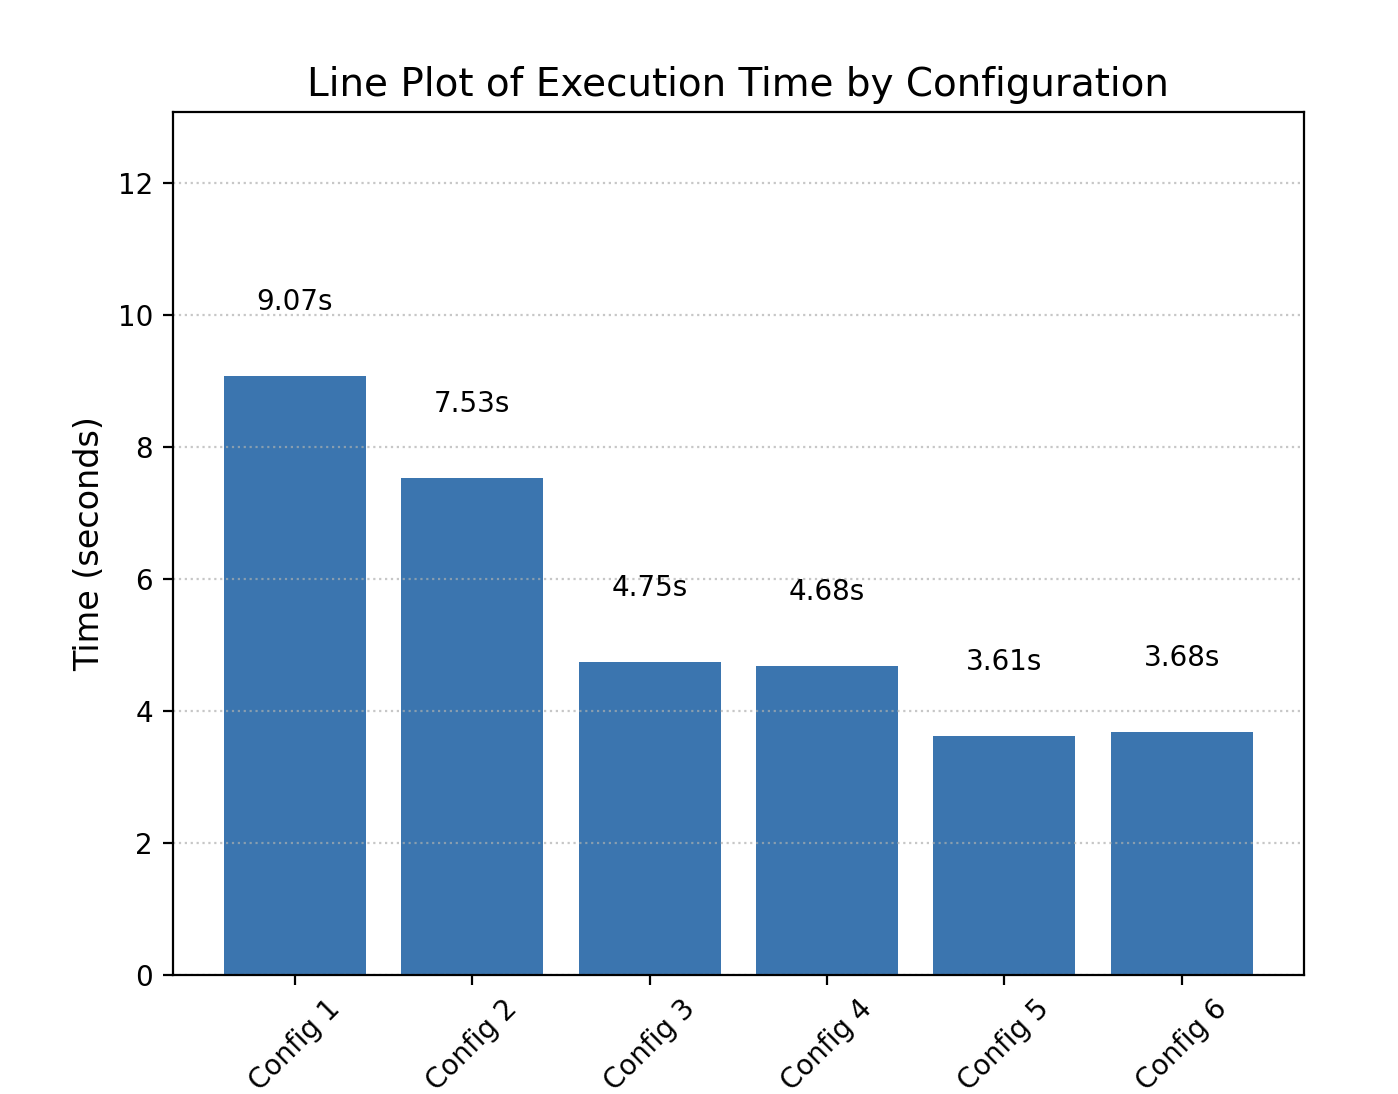
\includegraphics[width=0.46\textwidth]{TmalignBench.png}
    \caption{\label{fig:TmalignBench}Time taken for each configuration to run tmalign on 121 pairs of pdb files}
\end{figure}

\vspace{30px}

\begin{figure}[ht]
    \centering
    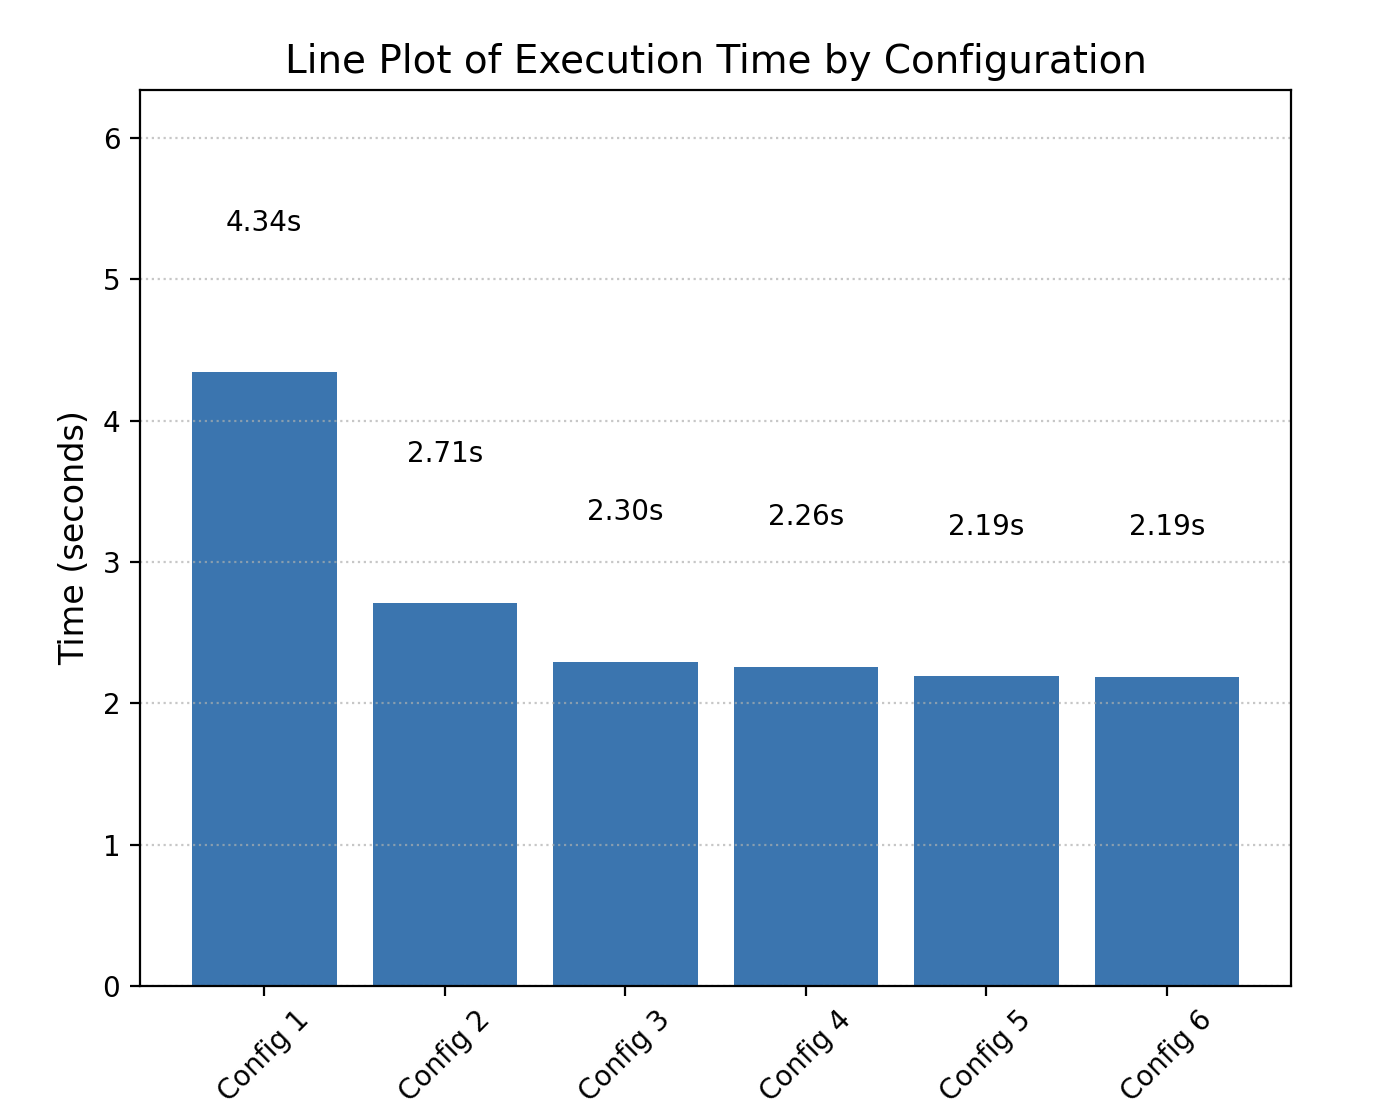
\includegraphics[width=0.46\textwidth]{linesBench.png}
    \caption{\label{fig:linesBench}Time taken for each configuration to run linecount on 161 pdb files}
\end{figure}

\vspace{15px}

The results will be discussed in section 7.2.




\clearpage

\subsection{Conclusion: Project Achievements}
To conclude, this section is created to discuss all the features that we accomplished whilst implementing the project. This included Pyspark, Cluset Setup, Key Value Pair, TMalign, API Service Download, Api Get and Benchmarking. We discuss each achievement explaining what they are. Ending the section with our benchmarking implementation. We go through our thought processes and display our results.

\section{Project Reflection}

Computational demands of analysing large datasets of protein structures can be a significant obstacle, requiring substantial time and resources. To address this challenge, this project aims to develop a framework that utilizes the MapReduce programming model to enable researchers to efficiently analyse large numbers of protein structures using a user-provided executable. To do this we have set out a list of objectives that once implemented will achieve the project aim. To do this we have conducted using python and spark. This enables the ability to parallelise data whilst computing a MapReduce step. As an outcome, all the objectives were implemented in a detailed manner except for the user interface. Overall the researcher can search and download pdb files from the framework. The researcher is also able to call out two user executables on the pdbs they require more specifically these are implemented using a MapReduce formalism. Whilst having some functions that help manipulate the folders holding the pdb files. Ultimately, at the end of this project, we have a software framework that supports MapReduce formalism and can process large numbers of protein structures. Whilst being able to do so by parallelising protein structure analysis across multiple computing nodes. Keeping in mind that the framework is optimized to reduce the processing time required for protein structure analysis. Finally, the software framework is scalable and can handle increasingly large datasets and can be easily updated to keep pace with advancements in protein structure analysis techniques and computing technology.

\subsubsection{Evaluate the process}

I had to amend the set-out deadlines I had created to better suit my priorities. These were the new deadlines created starting from week 1 shown in \ref{tab:Timeline}. This was because after completing my proof of concept programs I noticed that I was not collecting data from the pdb into a spark RDD in an efficient manner. Due to this, I took a technical decision to rethink and plan my priorities.

All set-out objectives were completed in order and according to the newly devised plan. However, setting up the cluster using the correct functions resulting in rdd and key-value pairs took more time than expected as at first I was trying to use just the data of the pdb file as the rdd. For this reason, I didn't have enough time to go back and create a good interface keeping at a bash level of interaction for the researchers. Due to this, I prioritise a more detailed readme file which helps the researcher understand the functions within the framework however a more user-friendly user interface would be beneficial for example when running the functions that implement the API to search or download pdbs a better user interface can be created that would be easier to use such as to set up the pdb files the researcher would like to run the executables on to.

\clearpage

\subsubsection{Improvements}
Looking back at the start of the project it would have been more beneficial if I conducted more research on spark and understanding the different RDD data types and functions available within spark would have meant that my spark cluster and RDD manipulation would have been efficient from the start. Due to this, I did not have time to implement the more complex JSON I created into my code more specifically not give the user the chance to modify/use the extra filters I spent time on creating a JSON for.

Another aspect I could have improved on is spending more time on the RCSB API documentation. I struggled and spent more time than expected creating a valid JSON for the API. This was due to being overwhelmed with the biology terms in the documentation so I sought out other means of creating the correct JSON for the API. One of these included looking through the requests being sent through the RCSB protein data bank website. Spending more time trying to understand the API documentation would have enabled me to complete the objective quicker and potentially create extra time for the user interface.

\vspace{40px}

\begin{table}[h!]
    \begin{center}
        \begin{tabular}{c|l|p{0.55\linewidth}}
        Week & Description & Explanation\\
        \hline
        \\
        1-2 & RDD setup & Create a better rdd setup within pyspark.\\
        \\
        \hline
        \\
        3-4 & RDD setup and Programs & With a better rdd setup apply these changes to the existing programs.\\
        \\
        \hline
        \\
        4-5 & Executables and Program & Find install and setup a suitable executable for protein structures and apply the executable to a cluster.\\
        \\
        \hline
        \\
        6-7 & Benchmarking & Setup and perform/document Benchmarking so that i can analyse performance depending cluseter configuration.\\
        \\
        \hline
        \\
        8-9 & Report & Start final report add in all privious work where need be and also include benchmarking.\\
        \\
        \hline
        \\
        10-11 & Extension and guidlines & Implement one extension whilst writing up some guidlines on how to run/use the executable\\
        \\
        \hline
        \\
        12 & Spark & Spare week\\
        \end{tabular}
        \caption{\label{tab:Timeline}The objectives I completed on a weekly basis}
    \end{center}
\end{table}


\subsection{Benchmarking Discussion}
In section 6 I have conducted benchmarking and show the results of the time taken to execute the user executables linecount and tmalign functions depending on the set configuration when creating the cluster. I showed all the different configuration sets and the time taken from each configuration more specifically the change of worker threads to available cores to complete its task. We discussed the differences between the two explaining how each effect cluster management. Before running the tests we were under the impression that the more worker threads and cores (max being the available cores on the machine) a configuration has we should have the faster the execution time. Looking at the graphs created we can conclude that this is true as time decreases every time we increase either option. Showing a strong correlation that the statement more cores and worker threads increase time efficiency.

\subsubsection{Configuration 1}
The first configuration contains one worker thread and one available core. This is a replicate of what the execution time would be if no parallelising was conducted. One key aspect of the project was to create a formalism that increases the efficiency of running multiple pdb files in parallel. We can see that this is correct as for both executables the time has significantly decreased as soon as more cores are available to the worker thread. We see a decrease of 1.53 seconds on the tmalign function and 1.63 on the linecount function when compared to Config 2. These differences are not so big due to the scale of the test set. However, increasing the test size should show a larger difference.

\subsubsection{Best Perorming Configuration}

Trying to conclude the best-performing configuration can be difficult due to the small test set. The best-performing configuration can also vary depending on the user executable being used for example adding a more intensive user executable might mean that a different configuration performs better than the rest. Out of the two executables, we can see that configuration 5 has performed the best this shows that having multiple worker threads that have more than one available core can utilize this and perform tasks the quickest. We see that in the linecount function configuration, 5 and configuration 6 performed the same. There can be several reasons for this but one reason I believe is that the function is not computationally heavy thus, having the extra available cores per worker thread did not make an impact on the performance.

\subsection{Conclusion: Project Reflection}
To conclude, we discuss our project reflection by re-stating the issue and our efforts in helping tackle it. We discuss the process of each aspect of the project explaining where we went wrong and how we overcame these issues and explaining the outcome of the decisions we made. We then move on to where we could have improved during our entire project and what that would have affected our project. Ending the section with a discussion on the benchmarking results comparing it to a non-parallel approach and deciding which configuration would be seen as the best performer.

\section{Professional Issues}
The use of complex data analysis methods and tools in structural bioinformatics necessitates a high standard of precision and dependability. As a result, it is crucial to take ethical considerations into account when discussing ethics within bioinformatics. It indicates that there may affect public health. Public health is a crucial aspect of structural bioinformatics since biological molecule analysis can improve our understanding of diseases and treatment alternatives. For instance, structural bioinformatics has been utilised to create new medications, vaccinations, and treatments that can enhance outcomes for public health.

Structural bioinformatics combines computational and experimental techniques to study the structure and function of biological molecules at a molecular level, requiring the analysis of large amounts of complex data and the use of advanced tools and techniques to extract
meaningful information.

The ethical concerns surrounding data privacy, ownership, sharing, informed consent,
and open science is crucial given the sensitive nature of the data involved.

\subsection{Data Privacy}

Structural bioinformatics deals with private information. The information that researchers obtain must be kept confidential and used only for the intended purpose. Whilst safeguarding against unauthorised access or disclosure. Requiring the use of secure storage methods or encryption to protect the data from unauthorised access ensures that any private information they collect is kept private and not disclosed to unauthorised parties. This will limit the impact on the exposed data, researchers must act swiftly in the event of a breach.

\subsection{Ownership}

Researchers must respect the rights of the individuals or organizations that provide the data and ensure that they are given appropriate credit for their contributions. As the researchers can exploit this for their own gain. In order to avoid this researchers need to obtain informed consent from participants before collecting their data, and clearly explain the purpose and potential risks of the study. The origin data provider should also be informed about their rights to access and control their data. Researchers must be transparent and should always make their findings public and be open about how they acquired the data. 

\subsection{Sharing of Data}

Sharing of data must be conducted responsibly and ethically, and having safeguards in place to protect the privacy and confidentiality of the data is necessary. We can avoid ethical issues here by establishing data sharing agreements for example, who has access to the data and how it can be used to protect the privacy and confidentiality of the data. An example can be removing personal information from the data, such as id or home address so we can not link it to particular people.

\subsection{Informed Consent}

Informed consent is obtaining permission from the provider after providing them with information about your intentions. This is important as it allows as it gives the provider an option on whether they would want to give consent.

When providing information to the provider the researcher must include:

\begin{itemize}
    \item Purpose of the data and intentions.
    \item Potential risks involved.
    \item Obtain written consent from participants.
\end{itemize}

\subsection{Open Science}

Open science is the practice of making research results and other outputs accessible to the general public and other scientists. This is crucial because it allows for peer review and the replication of research findings, which raises the quality and dependability of the study. Additionally, it encourages public trust and involvement by enabling access to and comprehension of research data. This increases collaboration and innovation in the area and produces new ideas and discoveries.

As it encourages accountability, transparency, and collaboration in research, open science is crucial to ethics. Gaining transparency and increasing trust with your participants and collaborators by making your study open and available to others. Ensuring that the research is carried out responsibly and ethically by holding yourself accountable to the scientific community and the general public makes the research transparent and accessible. Open science also encourages cooperation between institutions and researchers. Encouraging sharing of information and allowing a greater number of people to be benefited from findings.

\subsection{Conclusion: Professional Issues}
In conclusion, as the Structural Bioinformatics Framework is examined within the context of a MapReduce formalism, it is crucial to consider the ethical implications of this field. The potential impact of structural bioinformatics on public health is significant, but the responsible management of data privacy, ownership, sharing, informed consent and Open Science must be prioritized to ensure the ethical and responsible advancement of this field.

\section{Conclusion}
Overall, this dissertation project aimed to develop a software framework using MapReduce formalism for efficient analysis of large numbers of protein structures. The project set several objectives to achieve this aim, including developing a software framework that supports the MapReduce formalism, implementing a distributed computing system for parallelizing protein structure analysis, optimizing the software framework, designing an interface for manipulating the input data, ensuring scalability of the software framework, and integrating an API for PDB access. By achieving these objectives, the project aims to make a significant contribution to the field of structural bioinformatics, enabling researchers to analyze large numbers of protein structures more quickly and effectively than before.

The dissertation reviewed the literature of bioinformatics, spark/Hadoop, proteins, and their structures, and discussed the importance of the Worldwide Protein Data Bank in the field of bioinformatics. The project's implementation section discussed the setup of each user executable, the implementation of each objective, and the features that were accomplished, including Pyspark, Cluset Setup, Key Value Pair, TMalign, API Service Download, Api Get, and Benchmarking. The project reflection section discussed the process of each aspect of the project, where improvements could have been made, and the benchmarking results comparing parallel and non-parallel approaches.

It is crucial to consider the ethical implications of the field of structural bioinformatics, including data privacy, ownership, sharing, informed consent, and Open Science, to ensure the responsible advancement of this field. In conclusion, the Structural Bioinformatics Framework using a MapReduce formalism has the potential to significantly impact the field of bioinformatics and contribute to the analysis of large numbers of protein structures more efficiently.

\bibliographystyle{alpha}
\bibliography{bibliography}


\end{document}